%*************************************************************
\chapter{Scribbler}\label{ch:scribbler}
%*************************************************************

In den vergangenen Kapitel zeigten wir mit etlichen Beispielen wie und mit welchen Hilfsmitteln Gruppenmeetings abgehalten werden können. Sind es traditionelle Medien wie Papier und Flip-Charts, oder elektronische Medien wie computerunterstützte Whiteboardsysteme - sie alle finden Einsatz in Designsessions und bieten verschiedenste Vor- und Nachteile.

\medskip Im Folgenden wollen wir \scribbler vorstellen, ein elektronisches Interface, das die kollaborative Arbeit an virtuellen Artefakten unterstützen soll. Ähnlich wie die Autoren der bereits im ersten Kapitel beschriebenen Systeme, versuchten wir ein System zu kreieren, das die beiden Design-Arbeitswelten - geprägt durch traditionelle und elektronische Medien - mit einander verbindet und ihre Vorteile herausarbeitet. Im Gegensatz zu den bisherigen Ansätzen jedoch, ist \scribbler ein elektronisches Skizziersystem, welches ein barrierefreies Arbeiten ermöglicht.

\medskip Um dies zu zeigen, wollen wir vorerst, nach einer kurzen Beschreibung unserer Ausgangsituation, die Anforderungen eines kollaborativen Skizziersystems, die wir durch unsere Literaturrecherche gesammelt haben, zusammengefasst präsentieren. Danach werden wir die Vorgehensweise zur Erstellung unseres Prototyps schildern, welche selbst einige Designmethoden aus \autoref{ch:designTheorie} beinhaltet. Anschließend präsentieren wir die simple Oberfläche von \scribbler und dessen Funktionsumfang mit technischen Hintergründen. Zu guter Letzt stellen wir die Anforderungen und Merkmale gegenüber und beschreiben gewonnene Erkenntnisse aus Benutzererfahrungen.

\section{Ausgangssituation \& Rahmenbedingungen} \label{sec:ausgangssituation}
Die Technisierung vieler Berufe führte dazu, dass gewisse Arbeitsgegenstände ein elektronisches Abbild bekamen. Grafikdesigner beispielsweise fertigen heutzutage Präsentationszeichnungen, im Gegensatz zu früher, digital an. Neuere Berufsparten wie Interfacedesign setzen die tagtägliche Arbeit mit digitalen Artefakten vorraus. Wie schon in den vorigen Kapitel erwähnt, ist (im Besonderen) Design eine kollaborative Tätigkeit, wofür sich Gruppen zu Meetings treffen um gemeinsam neue Lösungen zu erarbeiten. Ein bewährtes und wichtiges Instrument dazu sind Stifte zur Erstellung von Skizzen, um Gedanken zu manifestieren.\\
Ein wesentlicher Bestandteil moderner Meetingräume ist ein zentraler Bildschirm oder Projektor, der als Präsentationsmittel verwendet wird. Zudem ist meistens eine Zeichenfläche vorhanden, wie z.B. Whiteboards oder Flip-Charts, um kollaborativ erarbeitete Ideen festzuhalten und neue Ideen zu explorieren.

\medskip Das Institut für Gestaltungs- und Wirkungsforschung an der TU Wien verfügt über so einen Meetingraum. Er besteht aus mehreren Tischen, die in der Mitte des Raumes zusammen gestellt wurden und um denen sich Sitzmöglichkeiten befinden. Neben einem Flip-Chart befindet sich ein {54\dq} großer Bildschirm in der Mitte einer Wand, auf den alle Meetingteilnehmer, von ihren Sitzplätzen aus, blicken können. Mit dem Screen ist ein Computer (Apple Mac Mini) verbunden, auf den Daten über ein drahtlos Netzwerk gespielt werden können. Eine zusätzliche drahtlose Tastatur und Maus ermöglichen eine bequeme Steuerung. Zusätzliche Peripherie kann auf der Rückseite des Computers angeschlossen werden.

\medskip Das Kerngebiet des Instituts ist \ac{HCI}, wodurch der Meetingraum oft dazu verwendet wird, Designs für interaktive Systeme, Applikationen oder Webinhalte zu erarbeiten. Ein Problem, das dabei erwartungsgemäß entsteht ist, dass bereits umgesetzte Inhalte nur digital vorhanden sind, was den Einsatz der wichtigsten Designmethode - Skizzieren - auf dem Artefakt fast unmöglich macht. Ziel unserer Arbeit war es nun ein Tool zu entwickeln, das es erlaubt, auf jegliche präsentierte Inhalte - seien es Webseiten, Programmoberflächen oder Bilder - >>kritzeln<< zu können. \scribbler soll so die Barriere zwischen der realen Welt und der digitalen Welt aufbrechen. \\Was benötigt man aber zur Umsetzung eines solchen Systems? Das wollen wir nun im nächsten Punkt kurz erläutern.

\section{Anforderungen an kollaborative Skizziersysteme} \label{sec:anforderungen}
Die letzten Kapitel gaben Aufschluss über das Verbesserungspotential vieler existierender Systeme. Wichtige literarische Größen auf diesem Gebiet, wie z.B. Lee, Olsen, Tang, Larsson, Johnson oder Prante, wiesen auf wesentliche Erkenntnisse hin, die ein solches System formen. Diese Erkenntnisse können vier großen Einflussfaktoren zugeordnet werden: \emph{Hardware}, \emph{Software}, \emph{Kollaboration} und \emph{Skizzieren} und bieten eine Art Checkliste für unser System. \autoref{fig:scribblerKollaborativesSkizziersystem} zeigt eine Aufstellung dieser Erkenntnisse, in Verbindung zu ihren Einflussfaktoren. 

\begin{figure}
	        {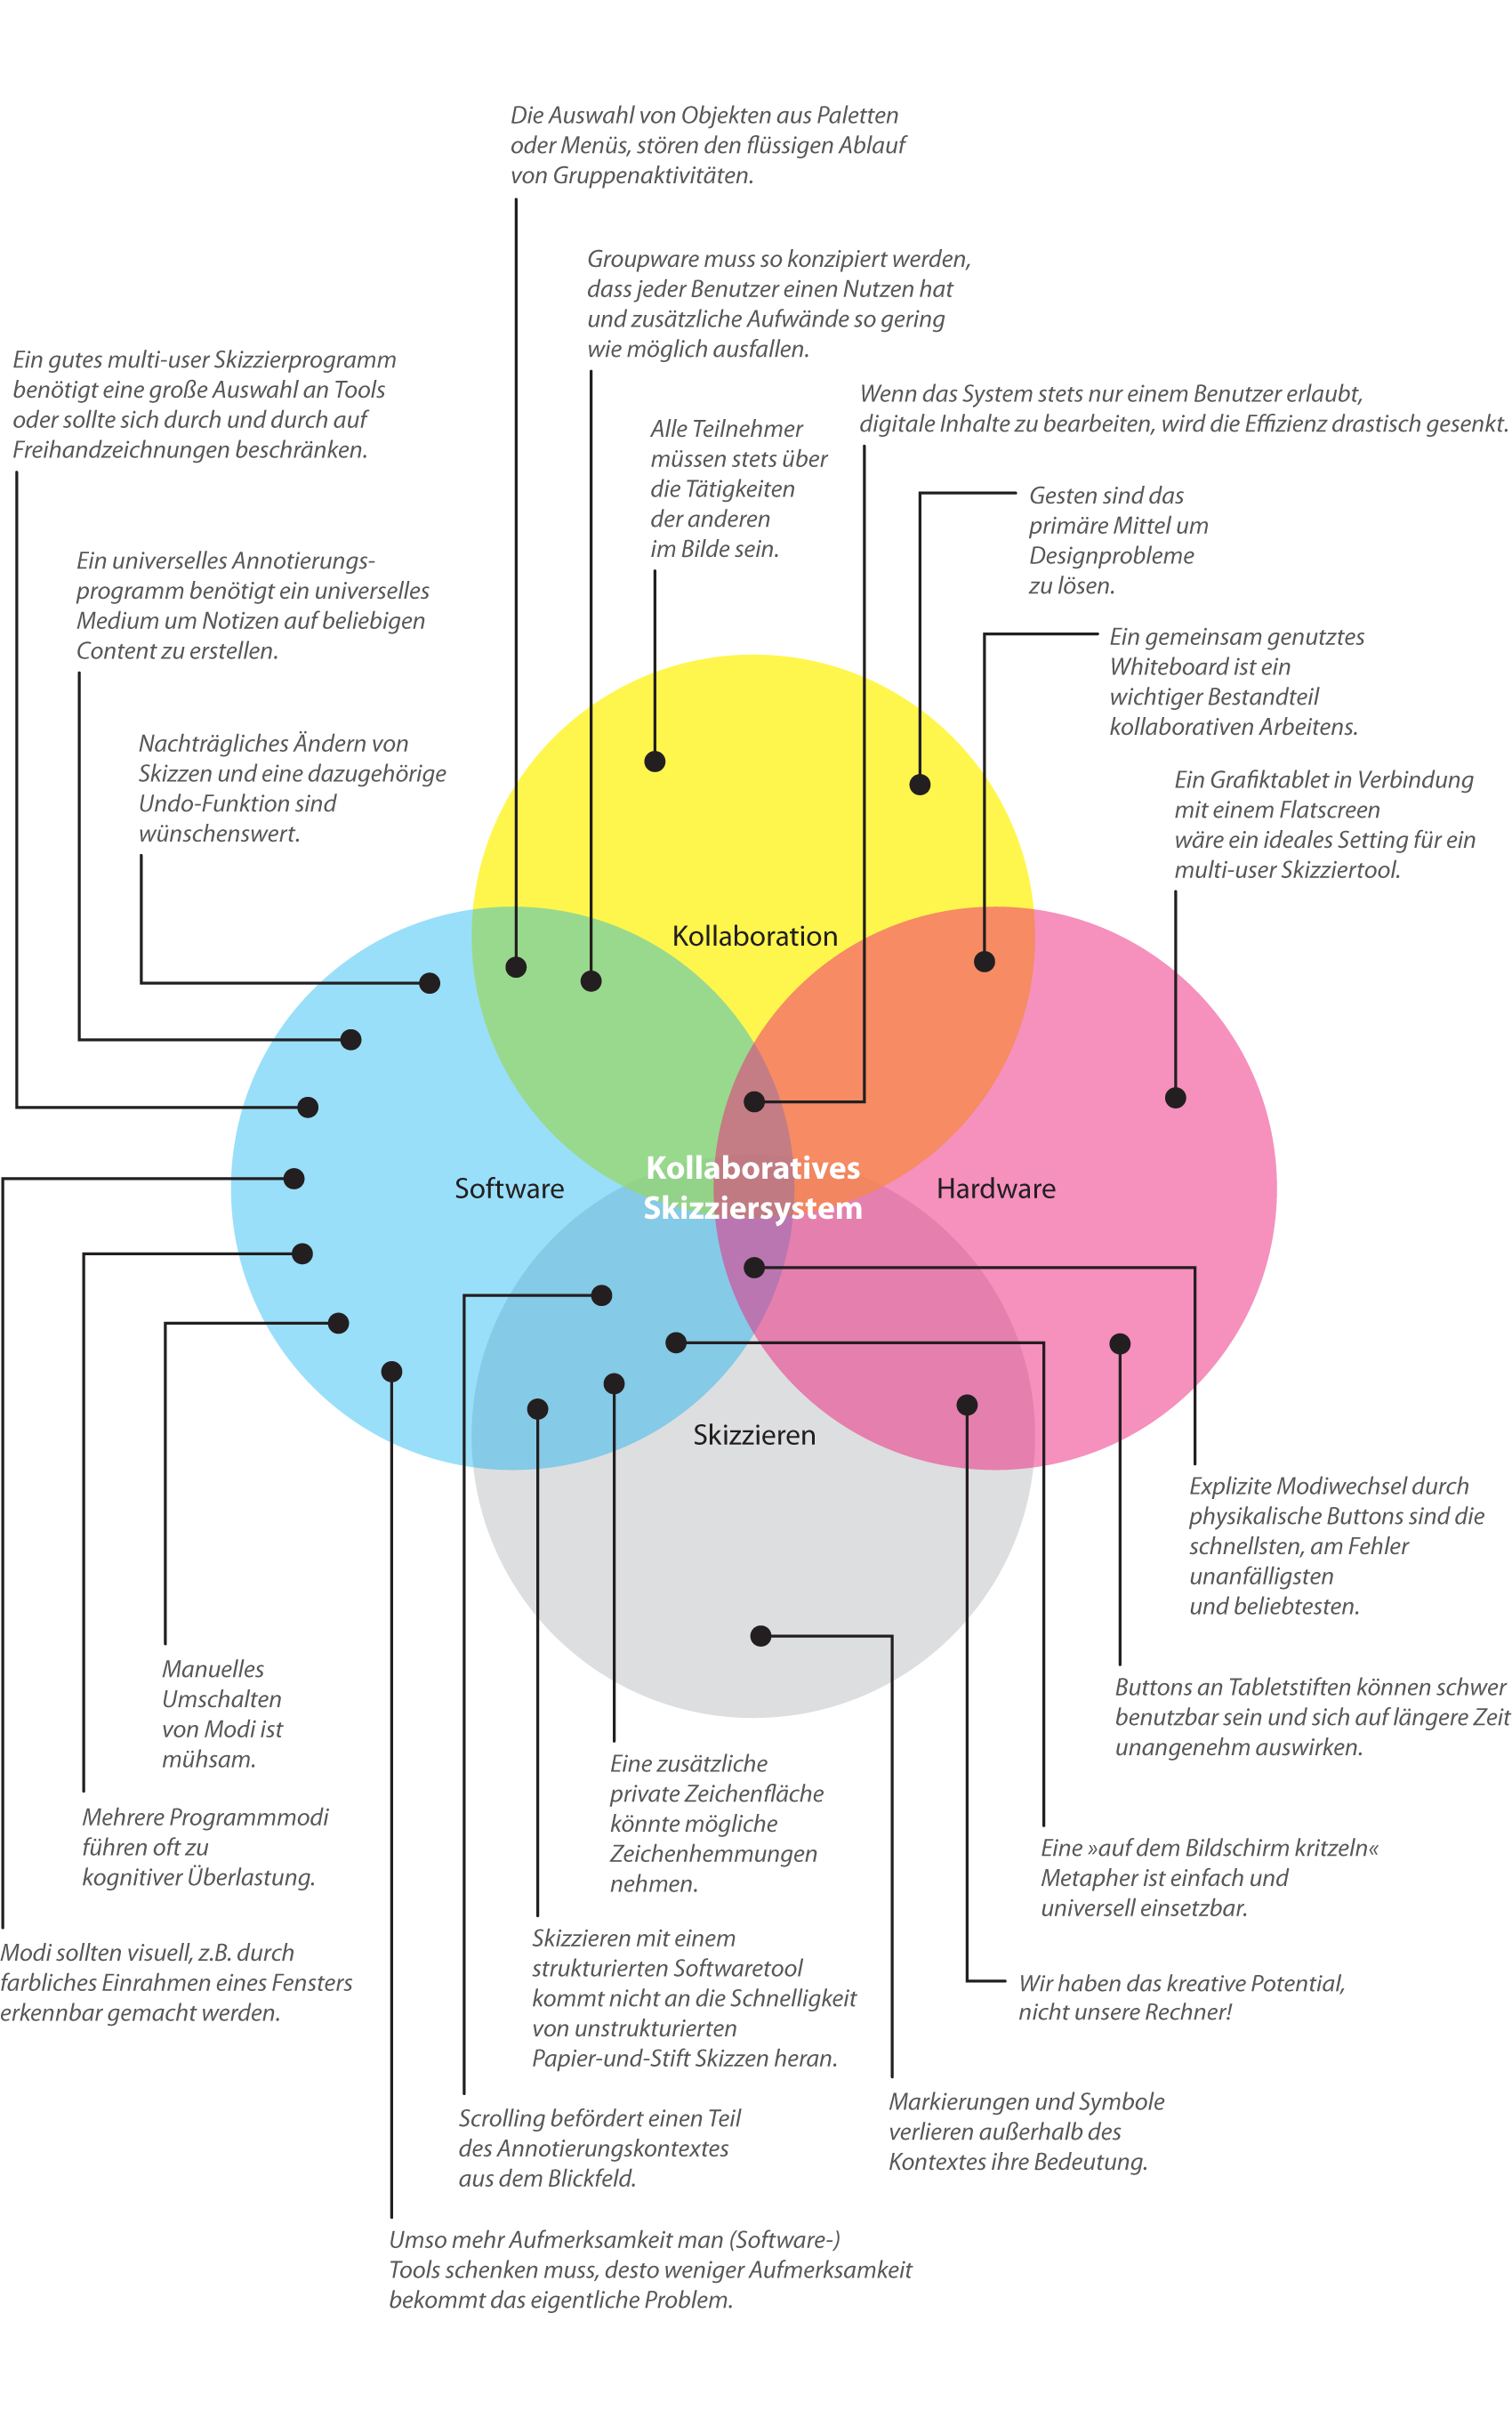
\includegraphics[bb=0cm 0cm 14.39cm 23.01cm]{gfx/scribblerKollaborativesSkizziersystem}}
		\caption[Anforderungen eines kollaborativen Skizzersystems]{Anforderungen eines kollaborativen Skizzersystems, bestehend aus den vier Einflussfaktoren: Hardware, Software, Kollaboration \& Skizzieren.}\label{fig:scribblerKollaborativesSkizziersystem}
\end{figure}

\medskip \emph{Hardware} Ein ideales Setting für ein kollaboratives Skizziertool wäre laut Lee ein Grafiktablet in Verbindung mit einem Flatscreen. Dies wäre die bestmöglichste Annäherung zu einer Technologie, die Stift und Papier ersetzen könnte. Sie würde ebenso zur Umsetzung eines Whiteboard Systems beitragen, was einen wichtigen Bestandteil kollaborativen Arbeitens ausmacht. Buttons an Tabletstiften können schwer benutzbar sein und sich auf längere Zeit unangenehm auswirken, deswegen sollte davon abgeraten werden diese mit einer Funktion zu belegen. 

\medskip \emph{Software} Ein gutes multi-user Skizzierprogramm benötigt eine große Auswahl an Tools, oder sollte sich durch und durch auf Freihandzeichnungen beschränken. Welcher Ansatz besser funktioniert, müsse laut Lee ausprobiert werden. Klar ist jedoch, dass umso mehr Aufmerksamkeit einem Softwaretool geschenkt werden muss, desto weniger Aufmerksamkeit bekommt das eigentliche Problem. Deswegen sollte solch ein System so simpel wie möglich aufgebaut sein. \\
Will man beispielsweise mehrere Programmmodi verwenden, muss man sich vor Augen führen, dass diese oft zur kognitiven Überlastung führen. Aus diesem Grund sollte der aktuelle Modus visuell, z.B. durch farbliches Einrahmen eines Fensters, erkennbar gemacht werden. Zudem ist das manuelle Umschalten von Modi mühsam. Es hat sich jedoch herausgestellt, dass explizite Modiwechsel durch physikalische Buttons, die schnellsten, am Fehler unanfälligsten und beliebtesten sind. \\
Will man ein universelles Annotierungstool schaffen, das über alle verwendeten Programme eines Benutzers funktioniert, benötigt man auch ein universelles Medium um Notizen auf beliebigen Content zu erstellen. Außerdem sind das nachträgliche Ändern von Skizzen und eine dazugehörige Undo-Funktion wünschenswert.

\medskip \emph{Kollaboration} Gemeinsam genutzte Systeme müssen so konzipiert werden, dass jeder Teilnehmer einen Nutzen hat. Wenn das System nur einen Benutzer erlaubt, digitale Inhalte zu bearbeiten, wird die Effizienz drastisch gesenkt. Zusätzliche Aufwände sollten so gering wie möglich ausfallen. Die Auswahl von Objekten aus Paletten oder Menüs, stören beispielsweise den flüssigen Ablauf von Gruppenaktivitäten. Die Teilnehmer der Kollaboration sollten ebenso stets über die Tätigkeiten der anderen im Bilde sein. Gesten spielen dabei eine wichtige Rolle.

\medskip \emph{Skizzieren} Das Zeichnen mit einem strukturierten Softwaretool kommt nicht an die Schnelligkeit von unstrukturierten Papier- und-Stift Skizzen heran. Eine >>auf dem Bildschirm kritzeln<< Metapher ist somit einfach und universell einsetzbar. Skizzen verlieren außerhalb des Kontextes ihre Bedeutung. Somit muss darauf geachtet werden, dass der Kontext stets bewahrt wird. Scrolling befördert z.B. einen Teil des Annotierungskontextes aus dem Blickfeld und benötigt somit zusätzliche Aufmerksamkeit bei der Umsetzung. Zudem könnte eine zusätzliche private Zeichenfläche mögliche Zeichenhemmungen von Teilnehmern nehmen. Alles in Allem haben wir das kreative Potential - ein Skizziersystem muss sich entsprechend adaptieren können.

\section{Vorgehensweise}
Nachdem wir erfuhren, dass Bedarf an einem elektronischen Skizziersystem bestand, begaben wir uns auf die Suche nach vergleichbaren Systemen. Dazu trafen wir uns für ein Brainstorming und explorierten verschiedene Begriffe, die uns zu dem Thema einfielen. In diversen Onlinedatenbanken fanden wir zu dazu Unmengen an Literatur und so Hinweise zu bestehenden kollaborativen Skizziertools. Nachdem wir die gesammelten Werke gemeinsam besprachen, erstellten wir ein vorläufiges Anforderungsprofil. \\
Eine wichtige Designfrage stellte sich schon zu diesem Zeitpunkt. Auf welche Eingabetechnologie sollten wir setzen? \autoref{fig:scribblerVorgehensweise} zeigt unsere Aufzeichnungen zu der wohl wichtigsten hardwarespezifischen Frage. Würden wir Skizzen erst nachträglich digitalisieren, wäre das System unabhängig von notwendigen Gerätschaften, was der Flexibilität des Systems zu Gute kommen würde. Jedoch ist es schwer gezeichnete Objekte nachträglich zu erkennen, wozu Mustererkennung notwendig wäre und das Ergebnis vielleicht nicht dem entspricht, was man eigentlich gezeichnet hat. Würden wir gleich auf digitales Zeichnen setzen, z.B. via Tablets, wäre die Flexibilität des Systems zwar eingeschränkt aber das Ergebnis akkurater. \\
Wir einigten uns, unter Absprache mit dem Institut, auf die zweite Variante, da Tablets bereits vorhanden waren und für einen ersten Prototypen ausreichen sollten.

\begin{figure}
	        {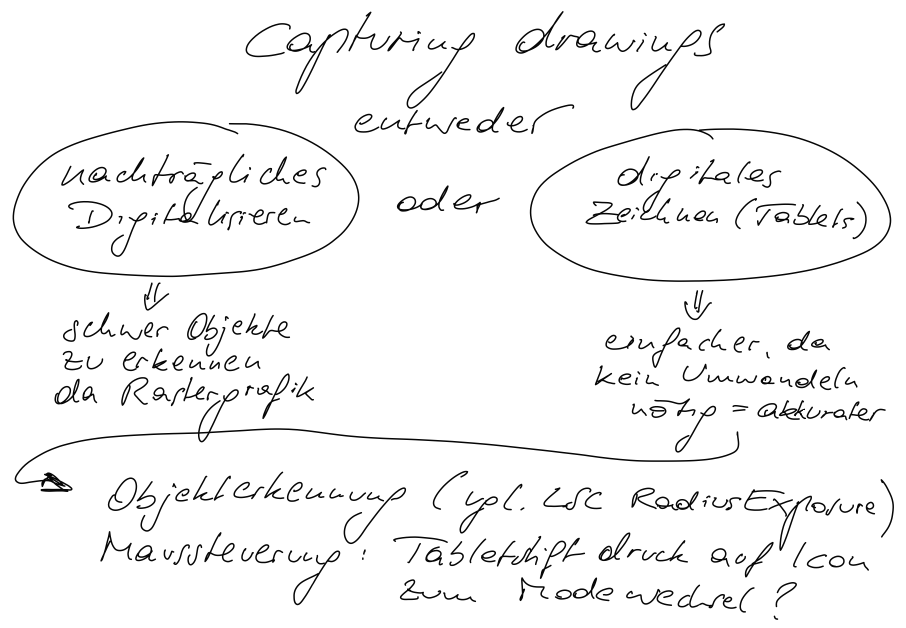
\includegraphics[width=1\linewidth]{gfx/scribblerVorgehensweise}}
		\caption[Aufzeichnung zur frühesten Designfrage]{Aufzeichnung zur frühesten Designfrage. Sollten Skizzen nachträglich digitalisiert werden oder sollte gleich auf digitales Zeichnen gesetzt werden?}\label{fig:scribblerVorgehensweise}
\end{figure}

Mit einem groben Konzept im Hinterkopf machten wir uns anschließend daran zu verstehen, wie skizziert wird. Dazu spielten wir selbst kreierte Szenarien mittels Skizzen durch. Später bauten wir simple Prototypen und versuchten das Skizzierverhalten unterschiedlicher Probanden zu analysieren. Nach einigen Tests konnten wir unser Konzept gering verfeinern, mussten aber gezwungenerweise frühzeitig damit beginnen, funktionellere Prototypen herzustellen. Da kein Mockup dieses stark verflochtene kollaborative Setting nachstellen könnte, begannen wir mit der Implementierung.

\bigskip \emph{Anmerkung: \graffito{\(\clubsuit\)} An dieser Stelle fiel erstmals der Begriff >>Scribbler<<, den wir weiters als Codenamen in unserem Projekt benutzten.}
\bigskip

Wir testeten jedoch fortlaufend unseren Prototypen, bis wir zu einem Punkt angelangten, an dem wir eine Betaversion unseres Programms definieren konnten, welches wir abschließend Userreviews unterzogen.

\medskip Wir wollen nun in den folgenden Punkten die angesprochenen verwendeten Designmethoden (vgl. \autoref{sec:designmethoden}) erläutern und mit Bildern untermalen. Sie sollen reichhaltiges Material zu Teilen des Designprozesses bieten, um auch diese durch praktische Beispiele zu konkretisieren.

\subsection{Recherche}
Recherchen gehören zwar nicht direkt zu Designmethoden, sind aber trotzdem ein wichtiger Teil in der Entwicklung eines Produkts. Durch Recherchen bringt man in Erfahrung, ob es bereits ähnliche Produkte oder Systeme auf dem Markt und in der Forschung gibt und bekommt gegebenenfalls einen Einblick in dessen Funktionsweisen.

\medskip Durch unsere Literaturrecherche fanden wir einige vergleichbare Systeme, mit der großen Einschränkung, dass Content und Input bisher nicht mit einander verknüpft werden. Es gibt zwar Annäherungen, jedoch bringen diese den Inhalt nur in eine statische Scheinbeziehung mit den Eingaben. Dies zeigte uns, dass wir auf dem richtigen Weg waren und der Bedarf eines neuen Skizziersystems, welches dieses Merkmal aufweisen würde, über die Grenzen des Instituts hinausgehen könnte. \\
Zusätzlich wies Literatur bereits auf Probleme hin, die durch die notwendige Selektion eines Werkzeuges entstehen können (vgl. \pointref{sec:ModusProblem}).

\medskip Die Recherchen wiesen uns in die richtige Richtung und ermöglichten uns neue Sichtweisen auf das geplante System, welche schließlich zum vorläufigen Anforderungsprofil führten.

\subsection{Skizzieren}
Das alleinige bzw. gemeinsame Skizzieren war das wichtigste Instrument in den Anfangsphasen von Scribbler. Skizzen ermöglichten uns Ideen zu veranschaulichen bzw. neue zu generieren und dienten somit auch als Diskussionsbasis. \\
Bei der Literaturrecherche fungierte meistens einer als Schreiber, der die wichtigsten besprochenen Fakten zusammengefasst in Stichwörter und kurzen Sätzen aufschrieb (vgl. \autoref{fig:scribblerVorgehensweise}). Skizzen wurden manchmal angefertigt um bestimmte Vorgehensweisen aus der Literatur zu illustrieren. Dies führte meist zu kollaborativen Arbeitsvorgängen, bei denen zusammen an einer Skizze gearbeitet wurde. 

\medskip Später wurden wie bereits erwähnt Skizzen zu wichtigen Szenarien erstellt. Eine farbliche Kennzeichnung war dabei oft sehr hilfreich. Zudem konnten Zugehörigkeiten oder zeitliche Abläufe durch Hinzufügen von Nummerierungen leicht angedeutet werden (siehe \autoref{fig:scribblerSzenarien}).

\medskip Abschließend zeigt \autoref{fig:scribblerDetailSkizze} ein Beispiel einer detaillierten Skizze, die dazu verwendet wurde um technische Abläufe zu verstehen. Sie entstand im Laufe der Entwicklung, in der ständig neue Ideen geboren wurden, welche durch Skizzen innerhalb des Teams erforscht wurden.

\begin{figure}
	\begin{center}
	        {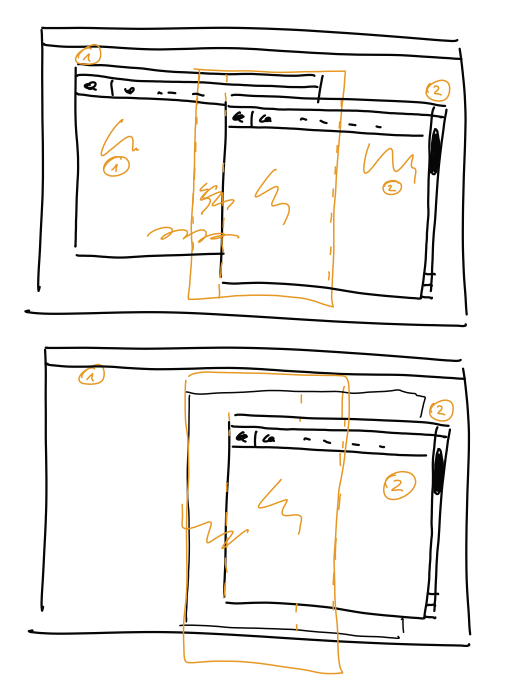
\includegraphics[width=0.8\linewidth]{gfx/scribblerSzenarien}}
		\caption[Skizzierte Szenarien in Scribbler]{Skizzierte Szenarien in Scribbler. Zugehörigkeiten wurden durch eine Nummerierung gekennzeichnet.}\label{fig:scribblerSzenarien}
	\end{center}
\end{figure}

\begin{figure}
	        {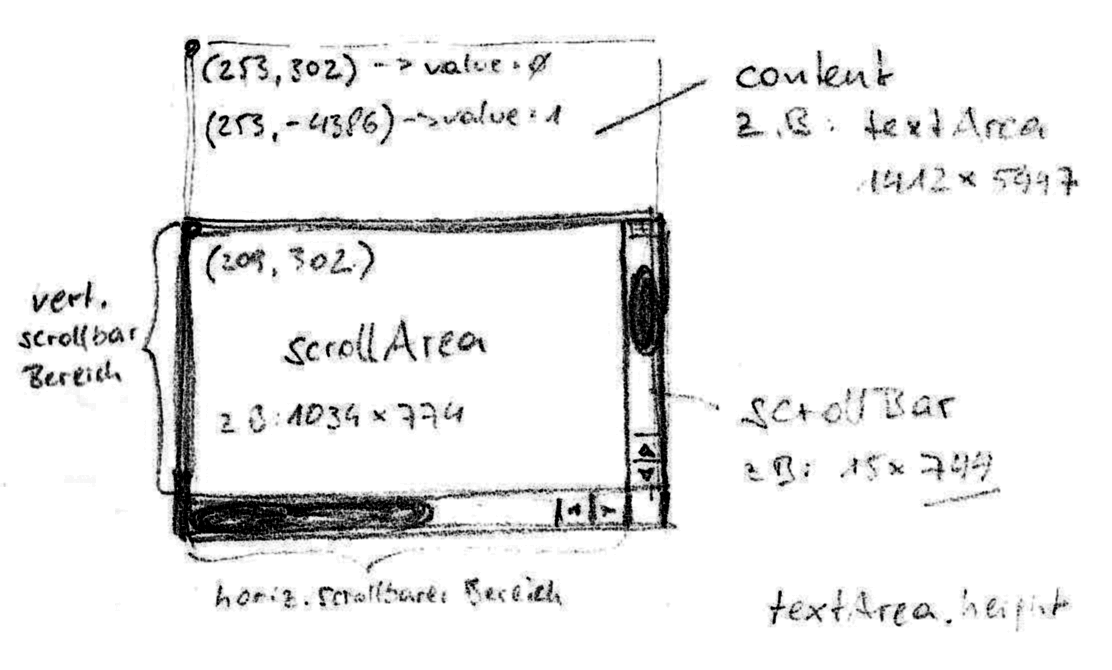
\includegraphics[width=1\linewidth]{gfx/scribblerDetailSkizze}}
		\caption[Detailskizze eines technischen Ablaufs]{Detaillierte Skizze eines technischen Ablaufs, um diesen besser zu verstehen.}\label{fig:scribblerDetailSkizze}
\end{figure}

\subsection{Prototyping}
Das Erarbeiten von Prototypen war keine leichte Aufgabe, da das Setting an sich, durch die verschiedenen Einflussfaktoren, kompliziert erschien. Dennoch konnten wir anfangs simple Prototypen, sog. Mockups bauen, um vorerst detailliertere Szenarien für uns zu erstellen und später das Skizzierverhalten einiger Probanden zu beobachten. Mockups sind low-fidelity Prototypen, wie beispielsweise auch Papierprototypen, die einen Wegwerfcharakter besitzen. Das bedeutet sie sind leicht zu Erstellen und bieten genug Funktionalität um Tests durchführen zu können.

\medskip \autoref{fig:scribblerMockups} zeigt ein Mockup, dass im Wesentlichen nur aus einem Screenshot eines \acs{WIMP}-Systems bestand (in unserem Fall Mac OS X mit zwei offenen Programmfenster) und in Verbindung mit einem Tablet PC benutzt wurde. Die für uns erstellten Szenarien, wurden durch den höheren Detailgrad konkreter, wodurch wir mehrere Funktionen im Voraus planen konnten. Später verwendeten wir diese dann um erste Tests durchzuführen. Der Prototyp beschränkte die Interaktionen der Benutzer auf das Skizzieren. So konnten wir beispielsweise feststellen, welche Plätze zum Zeichnen gesucht werden, wie bestimmte Elemente markiert werden oder Zusammenhänge von Inhalten hergestellt werden.

\begin{figure}
	        {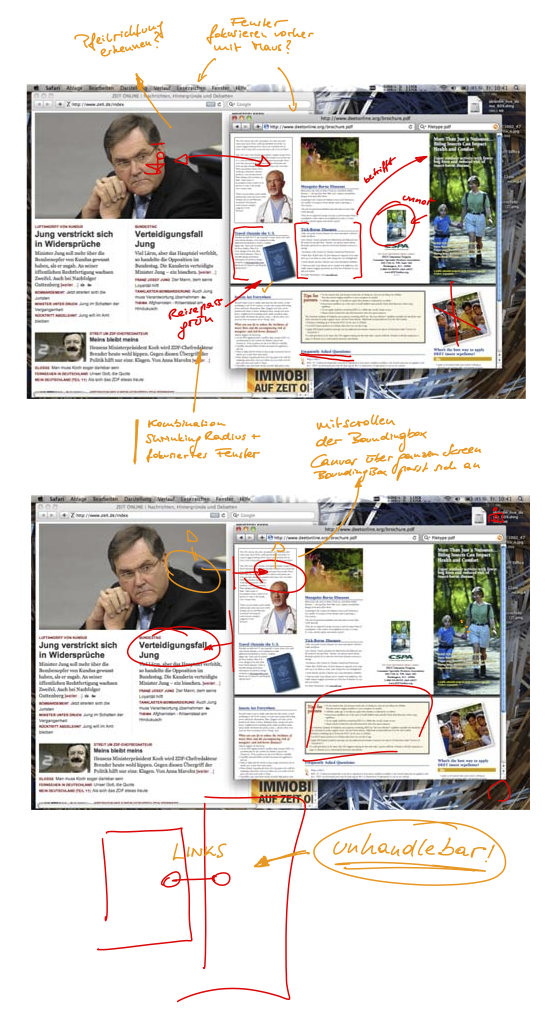
\includegraphics[width=1\linewidth]{gfx/scribblerMockups}}
		\caption[Mockups in Scribbler]{Simple Mockups, die durch Screenshots auf einem Tablet PC erstellt wurden.}\label{fig:scribblerMockups}
\end{figure}

\medskip Darauf folgende Prototypen waren ausprogrammierte Versionen von Scribbler, welche ebenfalls für Tests verwendet wurden.

\subsection{(User-) Testing}
Durch die erstellten Prototypen vor der Implementierung des Programms, war es möglich einen kleinen Funktionsteil mit Usern zu testen. Wichtige Systemverhaltensweisen bzw. Interaktionen konnten aber nur durch zusätzliche Testdurchgänge, während der Umsetzung, auf Verständlichkeit und Anklang geprüft werden.

\medskip Der Vorteil dieser Testdurchläufe, war die geringe Vorbereitungszeit. Es mussten keine bestimmten Anweisungen oder Aufgaben gestellt werden, da wir erstens die reale Welt um Bezug auf das Skizzieren mit Papier und Stift nachbilden wollten - was jedermann bereits in der Kindheit erlernt - und zweitens keine aufwändigen Aufgaben von Nöten waren. Probanden konnten einfach >>loskritzeln<<.

\medskip Wir hatten zudem die Möglichkeit \scribbler innerhalb einer Gruppe von fünf Personen zu testen, die an einem bestimmten Design arbeiteten und den in \autoref{sec:ausgangssituation} beschriebenen Meetingraum vom Institut dazu nutzten (siehe \autoref{fig:scribblerUserTest}).

\begin{figure}
	        {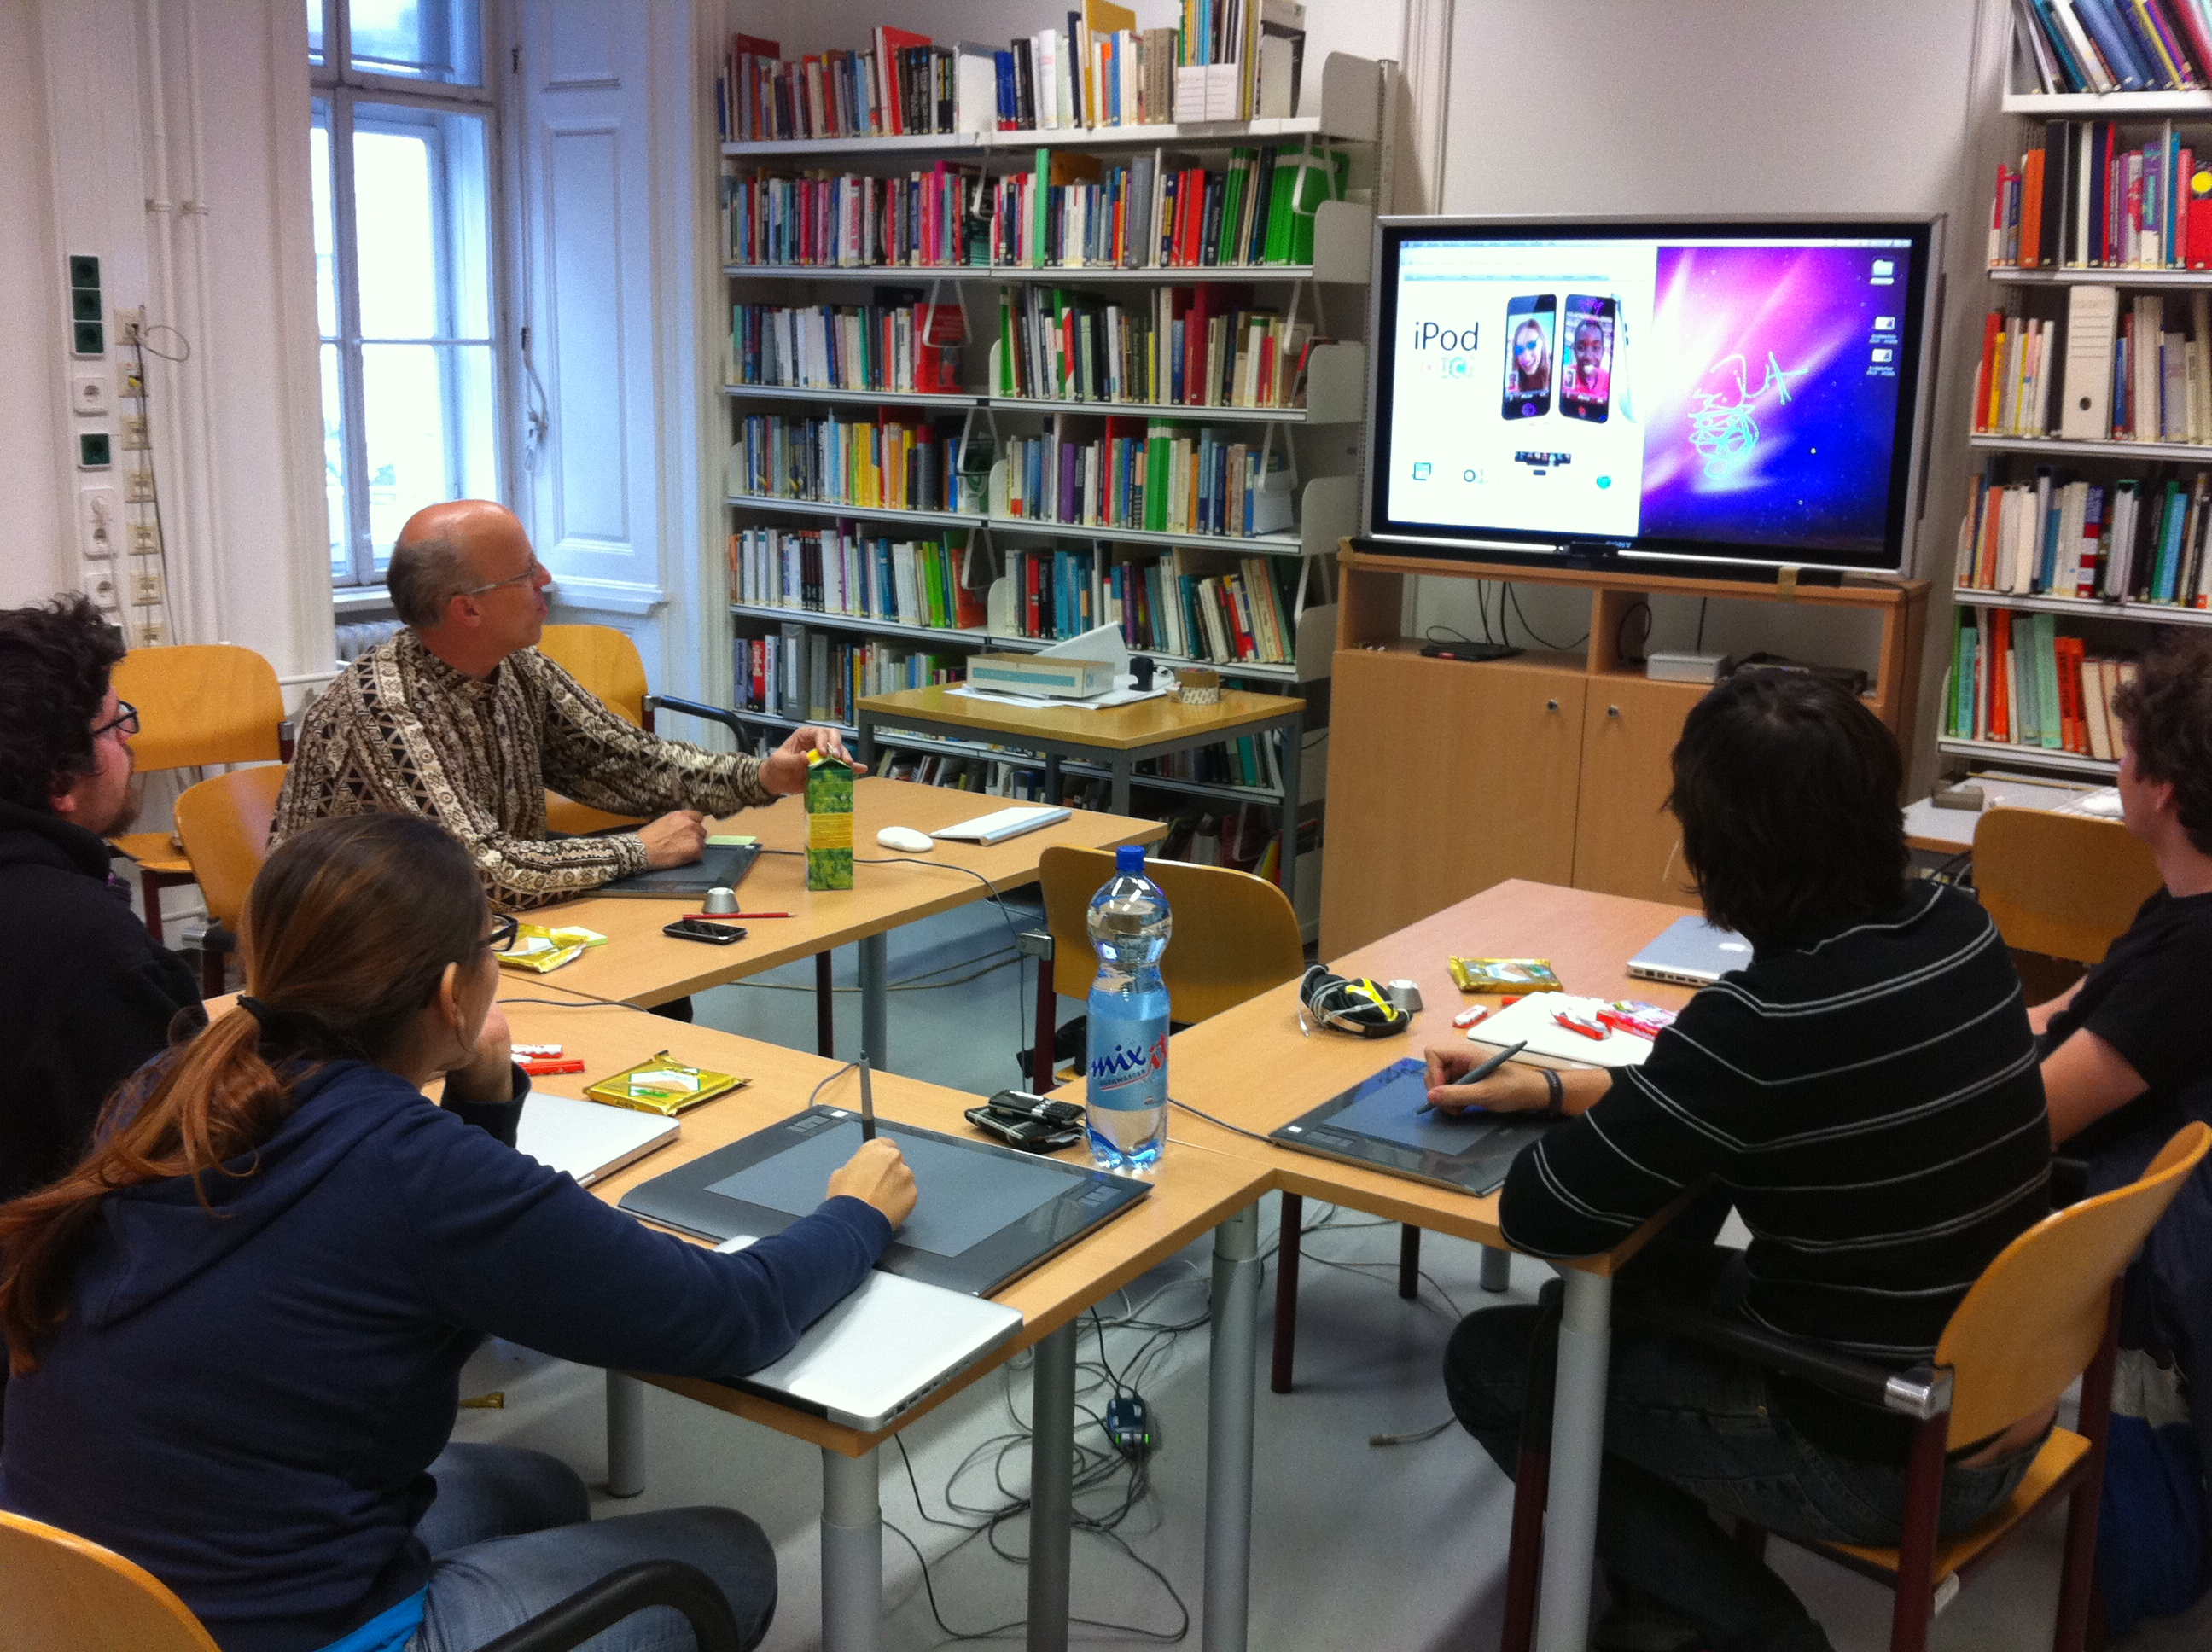
\includegraphics[width=1\linewidth]{gfx/scribblerUserTest}}
		\caption[Scribblertesting in einer Designsession]{Scribblertesting in einer Designsession. Fünf Personen überarbeiten mittels Scribbler ein Designvorschlag.}\label{fig:scribblerUserTest}
\end{figure}

\medskip Nach Fertigstellung der Betaversion, konnten wir \scribbler zusätzlich am Beginners's Day\footnote{Der beginners' day ist eine Infoveranstaltung für alle Studienanfängerinnen und Studienanfänger in den Informatik-, Wirtschaftsinformatik- und Lehramtsstudien. \citep{TU:2010}} der TU Wien vorführen und mit vielen erstsemestrigen Studenten testen. Abschließend konnten wir auch ausführliche Tests mit Designer durchführen, welche wir in \autoref{sec:userReview} ausführlicher beschreiben werden.

\section{Scribbler at a Glance}
Durch die verschiedenen Designmethoden, veränderte sich die Funktionalität von \scribbler öfters. Aus diesem Grund wollen unser Konzept  ordnungshalber erst jetzt anführen.

\medskip \scribbler ermöglicht neben der herkömmlichen Arbeit an einem Desktop (\acs{WIMP}) System, mittels Stiften auf jedes beliebige Programmfenster zu zeichnen. Das System läuft dabei im Hintergrund und aktiviert sich bei Bedarf. Wir unterscheiden dafür generell zwei Hauptmodi. Den Zeichen- und den Mausmodus. In letzterem kann die Maus wie gewohnt zur Navigation zwischen Programmfenster eingesetzt werden. Die Verwendung eines Tabletstifts hingegen wechselt in den Zeichenmodus. Die Benutzer können so auf das momentan aktive Fenster einer Drittapplikation >>kritzeln<<. Da besonders geübte Tabletbenutzer die Stifte auch als Ersatz für die Maus sehen, ermöglicht \scribbler auch das explizite Wechseln der beiden Modi durch Drücken einer Tablettaste.

\medskip Da beim Skizzieren natürlich auch Fehler auftreten können, bietet \scribbler eine \emph{Undo} bzw. \emph{Redo} Funktion. Versehentliche Änderungen können so rückgängig gemacht oder wieder hergestellt werden. Zudem können einzelne Striche gelöscht bzw. >>ausradiert<< oder der gesamte Zeichenbereich geleert werden.

\medskip Diese Grundfunktionalität soll vor allem Designer die Möglichkeit bieten, bestehende Arbeiten und Designs durchzubesprechen, Anmerkungen in direkter Verbindung zu digitalen Artefakten zu verfassen und kontextbezogene Erweiterungen zu zeichnen. Weil natürlich nicht immer schon vorhandene Designs vorliegen, bietet \scribbler aber auch eine Whiteboard Funktion. Dazu wird eine weiße Fläche über den gesamten Bildschirm eingeblendet, auf dem Benutzer Raum zum freien Skizzieren bekommen.

\medskip Um erarbeitete Skizzen zu speichern, besitzt \scribbler eine Screenshotfunktion. Nur durch Speichern eines Bildes, kann aus unserer Sicht der Kontext zu den Zeichnungen bewahrt werden. Will man Scribbler abschließend pausieren aber nicht beenden, kann man dies durch eine integrierte Standbyfunktion.

\medskip Die folgenden Punkte sollen nun nähere Informationen zu der Hardware, dem User Interface und dem logischen Programmaufbau geben. 

\subsection{Hardware} \label{ssec:hardware}
\scribbler benötigt ein relativ komplexes Hardware-Setting. Für die Ausgabe wird ein großes Display oder ein Beamer benutzt, während es für die Eingabe erforderlich ist, dass jeder Benutzer über ein Tablet mit Stift verfügt. Diese Tablets und das Ausgabegerät werden mit einem Rechner verbunden, auf dem das Apple Betriebssystem OS X 10.6 >>Snow Leopard<< läuft. Ältere Versionen von OS X werden von \scribbler nicht unterstützt. Für ein optimales Nutzungserlebnis, sollte der Computer über eine gute Rechenleistung verfügen. Bei der Umsetzung des Prototypen haben wir uns für Nutzung von Tablets aus der Modellreihe Intuos3 von Wacom entschieden. Diese Geräte verfügen über jeweils vier Buttons an beiden Seiten neben der Zeichenoberfläche, die mit verschiedenen Funktionen belegt werden können. Über diese Tasten können die folgenden Aktionen durchgeführt werden:

\begin{itemize}
	\item \emph{Wechsel des Interaktionsmodus für den Tabletstift}\\
	Ermöglicht das Umschalten von Zeichen- in den Mausmodus und umgekehrt. (Dies betrifft nur den Tabletstift, die Maus selbst ist immer im Mausmodus und kann nicht zum Zeichnen verwendet werden.)
	\item \emph{Whiteboard}\\
	Blendet eine weiße Fläche über den gesamten Screen ein oder aus. Auf dieser kann ebenfalls gezeichnet werden.
	\item \emph{Zurücksetzen}\\
	Löscht alle Zeichnungen des momentan aktiven Fensters.
	\item \emph{Sichern}\\
	Erstellt einen Schnappschuss des Desktops und der Zeichnungen des aktiven Fensters, der in einer Datei am Schreibtisch abgelegt wird.
\end{itemize}

\begin{figure}
	\begin{center}
        {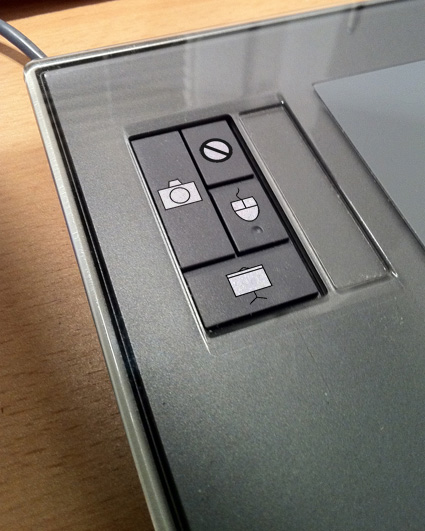
\includegraphics[width=0.8\linewidth]{gfx/scribblerTabletTasten}}
		\caption[Tablet Tastenbelegung]{Die Anordnung der \scribbler Funktionen auf den Tasten des Tablets. Der Fotoapparat links oben erstellt ein Bildschirmfoto, das Verbotszeichen auf der rechten, oberen Taste löscht alle Zeichnungen des aktiven Fensters, die Maus auf der genoppten, mittleren Taste wechselt den Interaktionsmodus und das Whiteboard auf der unteren Taste blendet selbiges ein oder aus.}\label{fig:scribblerTabletTasten}
	\end{center}
\end{figure}

\autoref{fig:scribblerTabletTasten} zeigt die Anordnung der Buttons auf den Tablets. Die mittlere Taste ist mit einer Noppe versehen und bietet dadurch ein haptisches Feedback. Dadurch kann der Button ertastet werden ohne dass ein Hinsehen von Nöten ist. Sinnvollerweise sollte diese Taste mit der wichtigsten Funktion belegt werden. In \scribbler ist dies der Wechsel des Interaktionsmodus, denn dieser ermöglicht, den vollen Interaktionsumfang mit nur einem Eingabegerät (dem Stift) zu nutzen. Die anderen beiden wichtigen Funktionen, sprich das Bildschirmfoto und das Whiteboard liegen auf den zwei großen Tasten links oben und unten. Das Zurücksetzen aller Zeichnungen wird relativ selten gebraucht und liegt daher auf der kleinen Taste rechts oben. Damit Benutzer diese Anordnung nicht auswendig lernen müssen, haben wir für Tests entsprechende Icons an den Tasten angebracht. Auf der rechten Seite der Zeichenoberfläche des Tablet sind die selben Tasten spiegelverkehrt angebracht, damit auch Linkshänder \scribbler optimal verwenden können.

\medskip Neue Wacom Tablets werden üblicherweise mit nur einem Stift ausgeliefert. In unseren Testsettings haben wir jedem Benutzer mehrere Stifte zur Verfügung gestellt. Diese haben alle eine Hardware-ID und können dadurch von \scribbler eindeutig identifiziert werden. So ist es möglich, dass jedem Stift eine eigene Farbe zugeordnet werden kann. \autoref{fig:scribblerColors} zeigt vier Stifte, denen unterschiedliche Farben zugeordnet sind. Um dies klar zu machen, haben wir jeden mit einem entsprechend gefärbten Sticker versehen. Der Wechsel zwischen Farben ist dadurch so intuitiv wie ein Farbwechsel beim Malen mit Buntstiften.

\begin{figure}
        {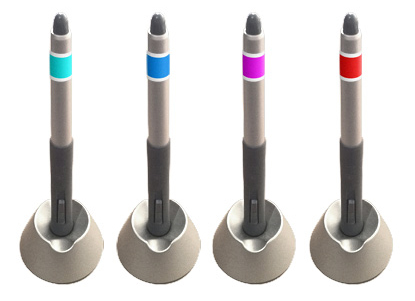
\includegraphics[width=1\linewidth]{gfx/scribblerColors}}
		\caption[Tabletstiftfarben]{Jeder Stift ist eindeutig vom System identifizierbar und hat eine eigene Farbe zugeordnet. Zur Verdeutlichung, wurde jedem Stift ein entsprechend gefärbter Sticker aufgeklebt.}\label{fig:scribblerColors}
\end{figure}

Jeder Stift hat einen Kippschalter an der Seite. Dieser erfüllt in \scribbler die Funktionen >>Undo<< und >>Redo<<, welche die letzte Aktion rückgängig machen oder wiederherstellen. 
%sDie Tests haben gezeigt, dass diese Buttons häufig unabsichtlich gedrückt wurden und daher in einer optimalen Version von \scribbler gar nicht mit Funktionen belegt werden sollten.
Stifte werden vom System erst dann wahrgenommen, wenn die Stiftspitze ein bis eineinhalb Zentimeter über das Tablet gehalten werden, wie \autoref{fig:scribblerProximity} demonstriert. Dies ist auf die Hardware zurückzuführen und es kann kein Einfluss darauf genommen werden. Ebenso wird das Drücken des Kippschalters am Stift nur dann registriert, wenn der Stift sich in der entsprechenden Entfernung zum Tablet befindet. Am hinteren Ende eines Stiftes befindet sich ein weiterer Button, der üblicherweise eine Radierfunktion bietet, ähnlich einem mit Radiergummi versehenen Bleistift. Auch \scribbler belegt diese Taste mit einer Radierfunktion, jedoch können damit nur komplette Linien gelöscht werden.

\begin{figure}
        {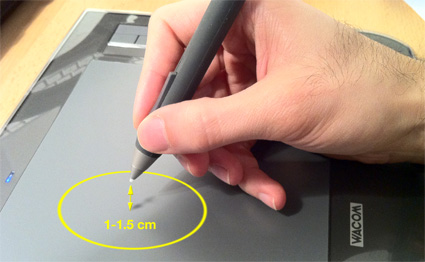
\includegraphics[width=1\linewidth]{gfx/scribblerProximity}}
		\caption[Proximity Event]{Die Hardware erkennt Stifte erst dann, wenn die Spitze ein bis eineinhalb Zentimeter über das Tablet gehalten wird. Das Betriebssystem empfängt dann ein >>Proximity Event<<, das von \scribbler weiterverarbeitet wird.}\label{fig:scribblerProximity}
\end{figure}

\subsection{User Interface}

\begin{figure}
	\begin{center}
        \myfloatalign
        \subfloat[Scribbler Icon]
        {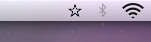
\includegraphics[width=0.47\linewidth]{gfx/scribblerIcon}} \quad
        \subfloat[When Magic happens..]
        {\label{fig:scribblerIcon}
        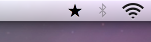
\includegraphics[width=0.47\linewidth]{gfx/scribblerMagic}} \quad
		\subfloat[Scribbler Menu]
		{\label{fig:scribblerMagic}
		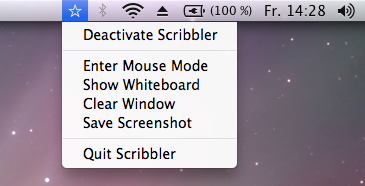
\includegraphics[width=1\linewidth]{gfx/scribblerMenu}} \\
        \caption[Scribbler Menu Icon]{Scribbler Menu Icon}\label{fig:scribblerMenuIcon}
	\end{center}
\end{figure}

\begin{figure}
        {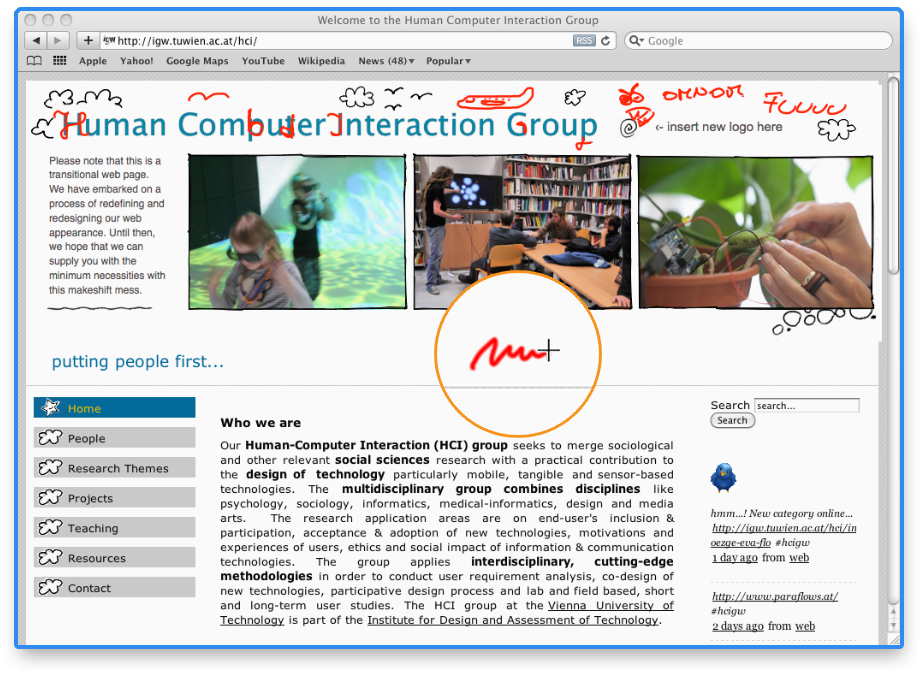
\includegraphics[width=1\linewidth]{gfx/scribblerSketching}}
		\caption[Skizzieren in Scribbler]{Skizzieren in Scribbler}\label{fig:scribblerSketching}
\end{figure}

\subsection{Programmlogik} \label{sec:programmLogik}
Blicken wir abschließend noch tiefer in die Materie. \scribbler wurde auf das von Apple entwickelte \emph{Cocoa}-Framework aufgebaut und genießt somit alle Vorteile einer objektorierten Programmiersprache. Zusätzlich bietet \emph{Mac OS X} eine Schnittstelle für Bedienungshilfen, sog. Accessibility Daten - aber mehr dazu später. Betrachten wir vorerst die Grundfunktionalität von \emph{Scribbler}.

\medskip \noindent \emph{Warum weiß Scribbler wann er in den Zeichenmodus wechseln soll?} \\
\scribbler fängt sog. globale und lokale Eingabe-\emph{Events} ab. \emph{Events} sind vom Benutzer hervorgerufene Aktionen, die an Eingabegeräten vorgenommen wurden. So ist ein Druck auf die linke Maustaste beispielsweise ein \emph{LeftMouseDownEvent}, oder das Halten einer Taste auf der Tastatur ein \emph{KeyDownEvent}. Auf die selbe Weise erkennt das System ein \emph{TabletProximityEvent}. Wie bereits im Punkt \pointref{ssec:hardware} ...
Voraussetzung ist, dass der Zeichenmodus aktiv ist.

\begin{lstlisting}[float,caption=Global and Local Event Monitoring]
// Start watching global events to figure out when to show the pane
	
[NSEvent addGlobalMonitorForEventsMatchingMask: (NSLeftMouseDraggedMask | NSKeyDownMask | NSKeyUpMask | NSTabletProximityMask | NSMouseEnteredMask | NSLeftMouseDownMask | NSOtherMouseDownMask | NSRightMouseDown | NSOtherMouseDownMask)
    handler:^(NSEvent *incomingEvent) {
	
    ...
}];

// Start watching local events to figure out when to hide the pane	

[NSEvent addLocalMonitorForEventsMatchingMask: (NSOtherMouseDownMask | NSRightMouseDownMask | NSKeyDownMask | NSKeyUpMask | NSTabletProximityMask)// | NSTabletPointMask)
    handler:^(NSEvent *incomingEvent) {

    ...
}];		
\end{lstlisting}

\begin{figure}
	\begin{center}
        \myfloatalign
        \subfloat[Mouse Position]
        {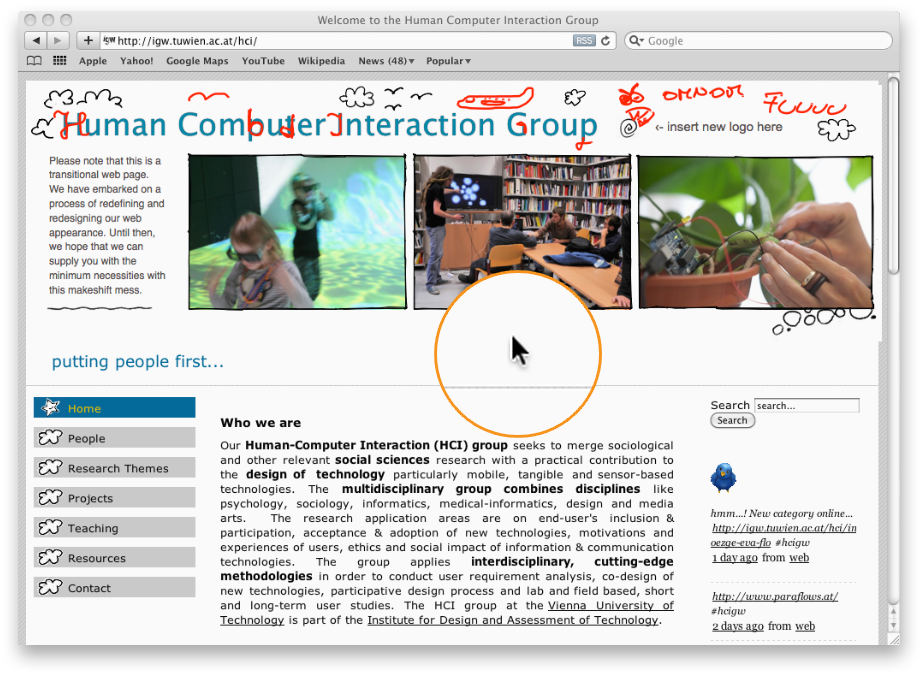
\includegraphics[width=1\linewidth]{gfx/scribblerAccessibility}} \\
        \subfloat[Accessibility Inspector]
        {\label{fig:scribblerAccessibilityInspector}
        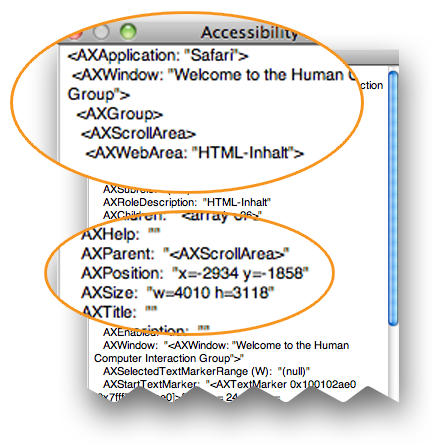
\includegraphics[width=0.7\linewidth]{gfx/scribblerAccessibilityInspector}} \\
        \caption[Accessibility Daten zur aktuellen Mausposition]{Accessibility Daten zur aktuellen Mausposition}\label{fig:scribblerAccessibility}
	\end{center}
\end{figure}

\begin{lstlisting}[float,caption=Laden von Accessibility Daten]
_systemWideElement = AXUIElementCreateSystemWide();
	
//Get the app that has the focus
AXUIElementCopyAttributeValue(_systemWideElement, (CFStringRef)kAXFocusedApplicationAttribute, (CFTypeRef*)&_focusedApp);

//Get the window that has the focus
if(AXUIElementCopyAttributeValue((AXUIElementRef)_focusedApp, (CFStringRef)NSAccessibilityFocusedWindowAttribute, (CFTypeRef*)&_focusedWindow) == kAXErrorSuccess) {
    ...
}		
\end{lstlisting}

\section{User Review} \label{sec:userReview}
Der Prototyp von \scribbler wurde von uns mit verschiedenen potenziellen Nutzern getestet. Darunter drei Designer aus den Bereichen Produkt-, Interaction-, und User Experience Design, die sich an \scribbler in einem reduzierten Setting, sprich mit nur einem Tablet versuchten. Zusätzlich setzte eine Arbeitsgruppe am Institut für Gestaltungs- und Wirkungsforschung der technischen Universität Wien \scribbler in einem kollaborativen Setting bei einem Projekt-Meeting ein. 

Bei allen drei Sitzungen wurden die Aktionen der Testpersonen durch eine Videokamera gefilmt und ihre Kommentare auf einem Tonträger festgehalten. Die drei Designer wurden zusätzlich von uns interviewt und die Transkripte sind im Appendix im Kapitel \nameref{ch:interviews} zu finden.

In den folgenden Abschnitten betrachten wir nun positives und kritisches Feedback, das aus diesen Tests hervorgegangen ist.

\subsection{Positives Feedback}

\scribbler wurde von den Testpersonen durchwegs positiv aufgenommen und alle waren interessiert an Konzept und Funktionsweise. Die Arbeitsgruppe am Institut für Gestaltungs- und Wirkungsforschung der technischen Universität Wien konnte den Prototypen produktiv bei ihrem Projekt-Meeting einsetzen und die Idee hinter \scribbler wurde als sinnvoll erachtet. 

Peter, seines Zeichens Produktdesigner und Dozent an der Universität für angewandte Kunst Wien, konnte sich sehr schnell mit \scribbler anfreunden und bewertete das Konzept sehr gut.

\begin{extract}[Peter, Produktdesigner, über \scribbler.]
	{
		\myfloatalign
		\begin{tabularx}{\textwidth}{p{1.5cm}X}
    		Peter  & Für mich ist das auf jeden Fall eine Traumsituation, da ich jetzt schon Notizen zu Präsentationen mache. Nur das Problem ist eben jetzt, dass ich die Notizen auf Zetteln mache und mir dazuschreiben muss, zu welcher Zeichnung die Notizen gehören, damit ich sie nachträglich wieder zuordnen kann.
		\end{tabularx}
	}
	\captionX{Traumsituation}
\end{extract}

Er könnte sich vorstellen, das Tool im Unterricht im kollaborativen Setting einzusetzen und erklärt, in welchen spezifischen Situationen \scribbler nützlich wäre und in welchen nicht.

\begin{extract}[Peter über den Einsatz von \scribbler im Unterricht.]
	{
		\myfloatalign
		\begin{tabularx}{\textwidth}{p{1.5cm}X}
    		Peter & Ja das wäre super, wenn ich das im Unterricht einsetzen könnte. Es wäre spitze wenn jeder die Möglichkeit hätte, mitzuarbeiten. Wobei ich nicht ganz sicher bin ob Darstellungstechnik das passende Unterrichtsfach für \scribbler ist, weil da geht es konkret um das Zeichnen und dann reichen Grobskizzen leider nicht aus, sondern man muss schon detaillierte Zeichnungen anfertigen. Anders sieht es da bei Designvisualisierungen aus, die auch in meinem Unterricht vorkommen. Da wäre es wirklich cool, die Studenten direkt einzubinden. Jeder könnte auch Stichworte dazuschreiben und ähnlich einem Brainstorming vernetzen. Das könnte ich mir gut vorstellen. 
		\end{tabularx}
	}
	\captionX{Einsatz im Unterricht}
\end{extract}

Jedem Stift eine eigene Farbe zuzuweisen findet Peter gut. Für seine Zwecke benötigt er mehr als nur eine Farbe und erscheint ihm eine gute Lösung. Er weist jedoch auch darauf hin, dass er gerne Kontextmenüs in Zeichenprogrammen verwendet und so schneller zwischen verschiedenen Farben wechseln kann.

\begin{extract}[Jedem Stift wird eine eigene Farbe zugewiesen.]
	{
		\myfloatalign
		\begin{tabularx}{\textwidth}{p{1.5cm}X}
    		Clemens & Du zeichnest derzeit mit der Farbe Magenta. Du hast vorher gemeint für Grobskizzen reicht dir eine Farbe oder?\\

			Peter & Also wenn ich in der Strukturierungsphase bin, wäre es schon gut wenn ich mehrere Farben hätte.\\

			Clemens & Ok. Dazu haben wir eigentlich mehrere Stifte mit unterschiedlichen Farben angedacht.\\

			Peter & Wirklich wahr?\\

			 & \emph{(Peter greift zu einem anderen Stift und probiert ihn aus)}\\

			Peter & Wahnsinn. Ja, das finde ich super wenn man das so löst.\\

			Thomas & Wir haben uns gedacht wir halten uns daran, möglichst realitätsnahe zu bleiben. Beim Zeichnen auf Papier würdest du auch einen anderen Stift zur Hand nehmen.\\

			Peter & Verstehe. Was ich irrsinnig gerne verwende sind Untermenüs bzw. Popupmenüs. Das gibt es bei verschiedenen Programmen. Wenn ich z.B. auf die Stifttaste drücke geht ein Untermenü auf. So wie bei >>Autodesk Maya<< oder >>Sketchbook<<. Das sind Programme in denen ich z.B. immer zeichne. Und da hätte man im Untermenü auch die Möglichkeit auf eine Farbpalette, oder vielleicht auch 2-3 verschiedene Strichstärken. Dazu drück ich auf die Stifttaste, fahre mit dem Stift auf das Menü, lass wieder aus, das Menü ist wieder weg und ich habe die neue Einstellung. Beim Zeichnen ist das super; das ist etwas was mir z.B. in Photoshop abgeht.
		\end{tabularx}
	}
	\captionX{Farben}
\end{extract}

Das Whiteboard, das in \scribbler eingeblendet werden kann und dazu dient, auf eine weiße Fläche statt einem bestimmten Fenster zu zeichnen, wurde von allen Testpersonen positiv bewertet. Es gibt Situationen, in denen man schnell etwas aufkritzeln möchte, das nicht mit dem Fensterkontext in Verbindung steht, beispielsweise eine spontane Idee für ein Konzept oder ein Design. In diesen Momenten bietet \scribbler die passende Funktion und die Idee kann so abseits vom aktuellen Geschehen festgehalten und später wieder abgerufen werden.

Durch \scribbler ist es möglich, auf mehrere nebeneinander angeordnete Fenster des Desktops zu zeichnen und dadurch semantische Verbindungen herzustellen. Dadurch können Inhalte auf eine ganz neue Art und Weise präsentiert werden. Momentan ist es so, dass Zeichnungen sich immer an das aktive Fenster, beispielsweise das Browserfenster heften und ihre Position relativ zur Fenster- und Scrollposition mitbewegen.

\begin{extract}[Zeichnungen heften sich an das aktive Fenster, auch wenn außerhalb dessen gezeichnet wird.]
	{
		\myfloatalign
		\begin{tabularx}{\textwidth}{p{1.5cm}X}
    		Thomas & Habe ich es richtig verstanden, dass du es gerne so hättest, dass wenn mehrere gleichzeitig zeichnen, jeder auf sein eigenes Fenster zeichnet und die jeweiligen Zeichnungen auf dem eigenen Fenster kleben bleiben? Momentan hängen alle Zeichnungen - egal von wem gezeichnet - nur auf dem aktivem Fenster. Sobald du das Fenster verschiebst, verschiebst du die Zeichnungen mit.\\

			 & \emph{(Peter denkt nach)}\\

			Peter & Weiß ich nicht. Also für mich funktioniert das derzeit von der Überlegung her recht gut. Aber ich müsste es erst länger ausprobieren, um auch die wirklichen Stärken zu finden.
		\end{tabularx}
	}
	\captionX{Zugehörigkeit}
\end{extract}

Als Produktdesigner zeichnet Peter wahnsinnig gerne und tut dies auch während er Besprechungen hält. Das Zeichnen hilft ihm mit den anderen zu kommunizieren und bringt seine Kreativität in Schwung. 

\begin{extract}[Zeichnen um besser zu kommunizieren.]
	{
		\myfloatalign
		\begin{tabularx}{\textwidth}{p{1.5cm}X}
			Peter & Was hier [in \scribbler] auch gut funktioniert, ist das Verdeutlichen von Ideen. Ich bin jemand, der irrsinnig gerne zeichnet zum Reden. Ich könnte so z.B. ein paar Punkte rausholen und einen Teil, der hier im Bereich unten schwer zu erkennen ist, noch einmal rauszeichnen.
		\end{tabularx}
	}
	\captionX{Kommunikation}
\end{extract}

Deshalb sieht er für \scribbler gute Einsatzmöglichkeiten bei Brainstormings und in Ideenfindungsphasen. Dadurch können Konzepte und Ideen schnell und effizient vermittelt und Inspiration gefördert werden. Ebenfalls denkbar wäre für ihn der Einsatz von \scribbler in Graphic-Recording-Meetings. Es handelt sich dabei um Sitzungen, bei denen eine Person jegliche verbale Kommunikation in der Gruppe als Skizzen festhält.

\begin{extract}[Ein Einsatz bei Graphic-Recordings wäre denkbar.]
	{
		\myfloatalign
		\begin{tabularx}{\textwidth}{p{1.5cm}X}
			Peter & Das ist eine recht interessante Geschichte. Es handelt sich um Leute, die Meetings mit zeichnen. Das passiert analog auf einem Blatt Papier mit Stift. Nehmen wir an da sitzen mehrere Techniker und andere in ein Projekt verwickelte Personen, die Konzepte verbal besprechen und dann gibt es einen Zeichner, der, während die Leute ihre Ideen artikulieren, diese direkt zu Papier bringt und aufzeichnet. Darauf baut dann die Diskussion weiter auf und die Teilnehmer können gleich auf die Skizzen eingehen und sie weiter entwickeln oder verwerfen. Am Ende kann man anhand der Bilder nachvollziehen, worüber gesprochen worden ist. Das wäre sicherlich auch ein Gebiet, bei dem man \scribbler oder ähnliche Anwendungen zum Einsatz bringen könnte.
		\end{tabularx}
	}
	\captionX{Graphic-Recording}
\end{extract}

\subsection{Kritisches Feedback}
Die Tests mit den potentiellen Benutzern haben nicht nur positive, sondern auch kritische Aspekte von \scribbler enthüllt. Einige davon waren uns bereits vor dem Testen bewusst und wurden durch die Tests und Interviews bestätigt, andere waren komplett neue Einsichten und haben uns auf wichtige Dinge aufmerksam gemacht. Die einzelnen Punkte haben unterschiedliche Gründe und werden im folgenden verschiedenen Kategorien zugeordnet, um ein besseres Verständnis zu bieten.

\subsubsection{Unvollständigkeit des Prototypen}
Als die Arbeitsgruppe am Institut für Gestaltungs- und Wirkungsforschung \scribbler in einem kollaborativen Setting beim Meeting einsetzte, war die erste Aktion der Benutzer logischerweise das Zeichnen. Alle griffen sofort zum Stift und wollten loslegen. Die Enttäuschung war groß, als sie realisierten, dass der Prototyp jeweils nur einem Benutzer zu zeichnen erlaubt, andere müssen warten, bis sie dran kommen. Uns war von Anfang an bewusst, dass dies eines der wichtigsten Features von \scribbler sein würde, aber leider war es uns nicht möglich, dieses in der kurzen Entwicklungszeit zu implementieren. Dieses Feature erfordert die Implementierung von multiplen Cursor und ist technisch aufwändig. Fehlt es jedoch, kommt es zu einem Flaschenhalseffekt, der die Effizienz von Meetings stark einschränkt. Personen können nicht parallel zeichnen, bzw. arbeiten und sind so ständig gezwungen, die Aktionen der anderen abzuwarten. Hinzu kommt ein erhöhter Aufwand der Absprache untereinander zur Koordination der Tätigkeiten. Der Test hat gezeigt, dass die Teilnehmer des Meetings sich ständig absprechen müssen, wer wann zeichnen kann. Dies ist eine Aktivität, die in herkömmlichen Meetings überhaupt nicht notwendig ist und stellt einen Nachteil gegenüber der Effizienz der Sitzung dar. Die Befürchtung, die wir bereits vor dem Test hatten, wurde sehr schnell bestätigt. Bei einer Weiterentwicklung von \scribbler muss diesem kritischen Feature höchste Priorität zugeordnet werden, denn es entscheidet über Erfolg oder Misserfolg des gesamten Systems.

\medskip Häufig kam es vor, dass Testpersonen unabsichtlich den Kippschalter am Stift drückten. Dies führte dazu, dass die letzte Aktion rückgängig gemacht wurde. Dieses Problem war uns schon während der Implementierungsphase bei internen Tests aufgefallen. Gerade Personen, die selten oder nie Tablet und Stift als Eingabegerät verwenden, passiert dieses unabsichtliche Drücken der Undo-Taste immer wieder. Der Produktdesigner, der täglich mit dem Tablet arbeitet, hatte hingegen keine Schwierigkeiten in dieser Hinsicht. Um \scribbler für eine breite Masse benutzbar zu machen, muss bei einer Weiterentwicklung darauf geachtet werden, dass den Tasten des Stifts keine Funktionen zugewiesen werden. Stattdessen sollten diese sinnvoll auf den Tasten des Tablets selbst angeordnet werden.

\medskip Es wurde sehr schnell deutlich, dass die Einsatzmöglichkeiten von \scribbler begrenzt sind. Die wenigen Zeichenfunktionen reichen lediglich für grobe Skizzen und Kritzeleien aus. \scribbler muss hier gezielt an Funktionalität angereichert werden und zumindest optional Features wie Strichstärke oder Druckempfindlichkeit anbieten.

\begin{extract}[Die Einsatzmöglichkeiten sind begrenzt.]
	{
		\myfloatalign
		\begin{tabularx}{\textwidth}{p{1.5cm}X}
			Thomas & Sind diese primitiven Zeichenmöglichkeiten ausreichend, oder fehlt dir da was?\\
			Peter & Nein, für Darstellungstechnik reichen diese Möglichkeiten bei weitem nicht aus. Man braucht da Dinge wie Strichstärke, gerade Linien, etc. Das sind Sachen, die Photoshop kann und die sind auch wirklich notwendig. Aber bei solchen groben Sachen, wie ich sie hier jetzt am Screen gezeichnet habe kann das schon reichen. Wichtig ist natürlich auch die Transparenz von Linien. Beim Skizzieren beginnt man ja mit ganz leichten Strichen, die das grobe Grundgerüst darstellen und zeichnet dann mit mehr Druckstärke drüber, sodass die Linien deutlicher werden und die Skizze konkreter wird.
		\end{tabularx}
	}
	\captionX{Fehlende Funktionalität}
\end{extract}

Der Prototyp war noch anfällig für Fehler und manchmal passierte es, dass das Programm komplett abstürzte oder unerwartetes Verhalten zeigte. Dies wurde zwar von den Teilnehmern bemängelt, jedoch zeigten alle Verständnis für die unfertige Teilimplementierung. Es ist jedoch klar, dass \scribbler in einer finalen Releaseversion absolut stabil laufen muss und nie Daten verlieren darf.


\subsubsection{Technische Probleme}
Eine große technische Hürde stellt für \scribbler das Speichern von Daten zur späteren Wiederverwendung dar. \scribbler hat natürlich keinen Einfluss auf andere Programme, hängt aber voll und ganz von deren Kontext ab. Das bedeutet, dass Zeichnungen in \scribbler nur dann sinnvoll sind, wenn die Fenster von Drittprogrammen darunter liegen. Die Problematik der Abspeicherung wird hier sehr schnell deutlich: \scribbler kann die Fenster und Anordnung von Drittprogrammen nicht speichern. Im Prototypen gibt es eine Funktion, die ein Bild vom Desktop mit allen Zeichnungen macht und in einer Datei am Schreibtisch ablegt. Dies ist natürlich ein Rasterbild und kann außer zum Ansehen kaum weiterverwendet werden. Zudem müssen bei längerem Arbeiten mit \scribbler sehr viele Bilder angefertigt werden, um alle Zeichnungen abzubilden. Dabei füllt sich der Desktop sehr schnell und zu einem späteren Zeitpunkt müssen Benutzer sich mit unzähligen Dateien plagen. Es muss hier dringend ein passendes Konzept gefunden werden, das die Bedürfnisse besser deckt als einfache Rasterbilder. 

\medskip Das Schreiben ist eine weitere Schwäche von \scribbler. Die prototypische Implementierung ist technisch nicht optimiert und das System zeichnet nur wenige Bewegungspunkte des Stifts am Tablet auf. Dadurch entstehen ungenaue Linien und Handschrift wird deutlich unlesbar. Gerade wenn Benutzer versuchen, auf kleine Flächen zu schreiben, scheitern sie in den meisten Fällen. \scribbler und der darunter liegende Code muss soweit optimiert werden, dass es möglich wird, auf Fenster in annehmbarer Größe zu schreiben, da dies ein sehr übliches Szenario darstellt.

\medskip Die Entscheidung, Tablets ohne integriertes Display als Hardware für \scribbler zu benutzen, fiel aus der Annahme heraus, dass Personen in kollaborativen Settings weniger miteinander interagieren würden, wenn jeder auf seinen eigenen Bildschirm starrt. Ziel war der Einsatz eines einzelnen großen Displays, um eine größere Gemeinsamkeit zu schaffen und Teamwork zu fördern. Vielen Benutzern fällt jedoch die Abstraktion von Tablet hin zu einem entfernten Display schwer. Sie schaffen es nur sehr schwer, ihre Bewegungen mit dem Stift am Tablet so zu koordinieren, dass am Display auch tatsächlich die beabsichtigten Striche gezeichnet werden. Bereits das Einkreisen von gewissen Elementen am Bildschirm kann quälend schwierig erscheinen und viel Frust beim Benutzer erzeugen. Diese Problematik verschärft sich, wenn das Display sich nicht frontal, sondern seitlich zum Benutzer befindet. Sitzt dieser dann auch noch schief vor dem Tablet, wird es schier unmöglich \scribbler sinnvoll zu nutzen.

\subsubsection{Konzeptionelle Probleme}
\scribbler setzt den Einsatz von spezieller Hardware voraus. Benötigt wird ein großes Display oder ein Beamer, ein starker Rechner mit dem Betriebssystem OS X und mehrere Wacom Tablets. Diese Komponenten sind zum einen teuer und zum anderen keine üblichen Geräte, die die meisten Betriebe im Inventar führen. Daher ist der Einsatz von \scribbler nicht ohne weiteres möglich, schon gar nicht vor Ort beim Kunden. Die ganze Ausrüstung dort hin zu transportieren stellt einen Aufwand dar, der in keinem Verhältnis zum effektiven Nutzen innerhalb eines Meetings steht.

\begin{extract}[Notwendige Hardware schränkt ein.]
	{
		\myfloatalign
		\begin{tabularx}{\textwidth}{p{1.5cm}X}
			Zed & \emph{[...]} Beim kollaborativen Zusammenarbeiten mit dem Kunden glaub ich nicht dass es funktionieren würde. Der Kunde kann das nicht bedienen, allein der Umgang mit dem Tablet ist eher komplex. Hinzu kommt die notwendige Hardware, die ja auch erst ein mal angeschafft werden muss und transportiert werden muss. Man benötigt dann ja mehrere Tablets. 
		\end{tabularx}
	}
	\captionX{Transport und Kosten}
\end{extract}

Für die Interaction- und User Experience Designer scheint \scribbler keine wirklich brauchbaren Szenarios und Einsatzmöglichkeiten zu bieten.

\begin{extract}[Der praktische Nutzen erschließt sich nicht jedem.]
	{
		\myfloatalign
		\begin{tabularx}{\textwidth}{p{1.5cm}X}
			Zed & Aber ich kann mir auch den praktischen Nutzen nicht so recht vorstellen. Zu sagen, ich würde das System wirklich irgendwo einsetzen... ich weiß nicht. Das Szenario fehlt mir. Beim Kunden fällt das nämlich komplett flach.
		\end{tabularx}
	}
	\captionX{Nutzen}
\end{extract}

Gewisse zusätzliche Features und Optimierungen würden das \scribbler Konzept jedoch interessanter für sie erscheinen lassen.

\begin{extract}[Notwendige Funktionalität.]
	{
		\myfloatalign
		\begin{tabularx}{\textwidth}{p{1.5cm}X}
			Thomas & Was wäre notwendig, um es für dich nutzbar zu machen?\\
			Zed & Dieser komischer Hovereffekt des Stifts am Tablet bereitet mir Schwierigkeiten. Das müsste man auf jeden Fall irgendwie lösen. Sodass man das Gefühl bekommt, dass man wirklich exakt arbeiten kann mit dem Ding. Das fehlt mir. Schön wäre natürlich auch, wenn man die Übersetzung von Tablet auf Screen lösen könnte, wobei das natürlich nur dann geht, wenn der Screen im Tablet integriert ist. Auch cool wäre, wenn man über das Internet zusammenarbeiten könnte, denn so ist man an dieses Setting im Raum gebunden, nicht mal über ein lokales Netzwerk hat man da irgendwelche Freiheiten.
		\end{tabularx}
	}
	\captionX{Nutzbar machen}
\end{extract}

Die Entscheidung, Linien in \scribbler als Vektorobjekte zu speichern, hat auch einige negative Nebenwirkungen mit sich gebracht. So ist zum Beispiel die Radiergummifunktion eingeschränkt. \scribbler kann immer nur eine ganze Linie komplett löschen. Das bedeutet, dass Striche mit dem Radiergummi nicht kürzer gemacht, sondern komplett gelöscht werden. Angenommen der Benutzer möchte wirklich nur eine Linie kürzen, die etwas zu lang geworden ist, so muss er sie löschen und neu zeichnen. 

\begin{extract}[Der Radierer löscht nur ganze Linien.]
	{
		\myfloatalign
		\begin{tabularx}{\textwidth}{p{1.5cm}X}
			Clemens & \emph{[...]} Die Möglichkeit zu Radieren gibt es eigentlich auch - die hintere Taste am Stift dient dazu. Doch da das Programm vektorbasierend ist, radiert es nur den letzten Strich. Ist diese Funktion zu wenig für deinen Gebrauch?\\
			Peter & Also wenn ich wirklich an einem Produkt arbeite, um eine Form herauszuarbeiten, wäre es zu wenig ja. Aber um einfache Sachen, wie z.B Notizen einzufügen oder Ideen zu formulieren, funktioniert es schon. Man müsste aber vielleicht anfangen das Programm häufiger zu verwenden, um ein gutes Feedback abgeben zu können.
		\end{tabularx}
	}
	\captionX{Radieren}
\end{extract}

\subsubsection{Wünsche der Benutzer}
Offensichtliche Verbesserungen, wie Druckempfindlichkeit, Strichstärke und generell konkretere Zeichenmöglichkeiten wurden von fast allen Teilnehmern angesprochen. Zusätzlich gab es einige Einwände und Ideen zu Features, die das Nutzungserlebnis von \scribbler verbessern könnten. Essenziell für ein effizientes Arbeiten mit \scribbler erscheint die Möglichkeit, Zeichnungen nachträglich am Bildschirm noch verschieben zu können. So können erst Ideen generiert und danach Ordnung und Struktur geschaffen werden.

\begin{extract}[Es wäre gut, wenn man Zeichnungen verschieben könnte.]
	{
		\myfloatalign
		\begin{tabularx}{\textwidth}{p{1.5cm}X}
			Thomas & Ich habe gesehen, du würdest dir auch wünschen dass du einzelne Teile von Zeichnungen wo anders hinschieben könntest oder? Also dass du einen bestimmten Bereich ausschneiden und verschieben könntest.\\
			Peter & Ja, das wäre vielleicht speziell bei der Ideenfindung, wo alles durcheinander steht, oder auch bei Skizzen in einem Brainstorming technischer Natur interessant. Weil meistens ist der zweite Schritt dann der, dass ich anfange die Ideen zu ordnen. Also es wäre gut, um den ersten Prozess der Ideenfindung nicht zu stoppen bzw. ihm eine Hürde zu geben, sondern gleich weiterarbeiten zu können. Und da ist es eben notwendig das Ganze in eine Ordnung zu bringen. Dann hätte ich wirklich eine Lösung wo alle gemeinsam arbeiten können.
		\end{tabularx}
	}
	\captionX{Verschieben}
\end{extract}

Pi und Zed hatten die Idee, zusätzlich ein Trackpad anstatt einer Maus zusammen mit dem Tablet als Eingabegeräte zu nutzen. Das Tablet wäre nur für Schreiben und Zeichnen zuständig, während das Trackpad zu Positionierung des Cursors genutzt werden könnte. Eventuell würde man so die Steuerung für Benutzer optimieren, die im Umgang mit Tablets ungeübt sind.

\begin{extract}[Ein Trackpad statt einer Maus könnte die Eingabe erleichtern.]
	{
		\myfloatalign
		\begin{tabularx}{\textwidth}{p{1.5cm}X}
			Pi & Vielleicht ist die relative Projektion des Tablets dann sinnvoll, wenn man zwei Eingabegeräte verwendet. Dann setze ich mit der Maus den Zeiger dorthin, wo ich ihn möchte und kann sofort dort los zeichnen, egal wo am Tablet sich mein Stift befindet. \emph{[...]} Oder man könnte auch überhaupt zwei Tablets haben, das eine zur Steuerung mit Gesten und das andere zum Zeichnen.\\
			 & \emph{[...]}\\
			Zed & Da würde sich doch das Magic Pad von Apple anbieten.
		\end{tabularx}
	}
	\captionX{Trackpad}
\end{extract}

Von allen drei Designern wurde der Wunsch nach einer Online-Funktion geäußert. Sie alle haben schon öfter die Erfahrung gemacht, mit anderen Kollegen über das Internet zusammenzuarbeiten und es würde sich anbieten, \scribbler dafür zu nutzen. Für die lokale Benutzung würden sich die beiden auch wünschen, dass nicht nur die Zeichnungen des aktiven Fensters sondern jene von inaktiven Fenstern im Hintergrund angezeigt werden. Um Chaos auf dem Bildschirm zu vermeiden könnte man beispielsweise Zeichnungen im Hintergrund in Grau und mit verschiedenen Alpha-Werten, entsprechend dem Z-Index des zugehörigen Fensters anzeigen.

\begin{extract}[Es sollten nicht nur Zeichnungen des aktiven Fensters dargestellt werden.]
	{
		\myfloatalign
		\begin{tabularx}{\textwidth}{p{1.5cm}X}
			Zed & Das heißt es hängt alles an einem Fenster dran... hmmm, kannst du mal bitte das hintere Fenster aktivieren und es so verschieben, dass man die Fenster und Zeichnungen dahinter sieht?\\
			Thomas & Hmm, das geht so nicht. Es werden immer nur die Zeichnungen auf dem aktiven Fenster angezeigt.\\
			Zed & Ah, hmm. Ich glaub das irritiert mich, dass die Zeichnungen verschwinden. Vielleicht sollte man die ausgegraut anzeigen, so wie die inaktiven Fenster selbst.\\
			Clemens & Es besteht dann die Gefahr, dass ein Chaos entsteht, wenn zu viele Linien angezeigt werden.\\
			Zed & Ja stimmt, aber man könnte doch mit verschiedenen Alpha-Werten arbeiten, je nach dem, wie weit hinten sich ein Fenster befindet.\\
			Thomas & Oh, ja das klingt nach einer guten Idee.\\
			Pi & Man könnte dadurch den Kontext wahren und sehen was man bereits gemacht hat.
		\end{tabularx}
	}
	\captionX{Inaktive Fenster}
\end{extract}

Zudem kam bei ihnen der Wunsch nach einer besseren Darstellung der Zugehörigkeit von Zeichnungen zu Fenstern auf. Eine Idee wäre Farbe dafür einzusetzen, jedoch würde dies wiederum die Freiheit beim Zeichnen einschränken, da keine beliebigen Farben mehr gewählt werden können. Auch eine Darstellung, wer welche Zeichnungen gemacht hat, sollte es geben. Im Testsetting, das die Arbeitsgruppe an der Universität eingesetzt hat, wurde dies so gelöst, dass jedem Tablet eine Farbe zugewiesen wurde. Zu jedem gab es mehrere Stifte, die unterschiedliche Helligkeitswerte mit dem Farbwert des Tablets kombinierten. So konnte zumindest etwas Variation eingebracht werden. Im kollaborativen Setting wäre es ebenfalls wünschenswert, wenn mehrere Benutzer gleichzeitig auf verschiedene Fenster zeichnen könnten und die Zeichnungen dem jeweiligen darunter liegenden Fenster zugeordnet werden könnten. Dies stellt natürlich eine große technische Hürde dar und bei einer Weiterentwicklung von \scribbler muss die Machbarkeit erst exploriert werden.

Peter, der Produktdesigner, würde außerdem ein Kontextmenü benötigen, das ihm ein paar Optionen anbietet. Gängige Skizzierprogramme bieten diese Funktion an und ermöglichen so eine sehr hohe Effizienz bei der Arbeit.

\section{Achievements}
Abschließend wollen wir nun kurz die in \autoref{sec:anforderungen} beschriebenen Anforderungen an ein kollaboratives Skizziertool, mit den umgesetzten Merkmalen von Scribbler gegenüberstellen und somit auswerten. Wiederum teilten wir die Merkmale von Scribbler in die vier Einflussfaktoren: \emph{Hardware}, \emph{Software}, \emph{Kollaboration} und \emph{Skizzieren}.  \autoref{fig:scribblerAnforderungsauswertung} veranschaulicht diese durch eine farbliche Kennzeichnung der ursprünglichen Erkenntnisse aus der Literatur. In Grün gehaltene Erkenntnisse wurden in der Betaversion von \scribbler bereits behandelt, rot eingefärbte konnten (noch) nicht umgesetzt werden.

\medskip Wie die Abbildung erkennen lässt, konnte ein Großteil der Anforderungen umgesetzt werden - um genau zu sein 17 (77,27\%). Die restlichen 5 (22,73\%) blieben vorwiegend durch technische Probleme bis dato ungelöst.

\medskip \emph{Hardware} Durch das Benutzen von Grafiktablets in Verbindung mit einem Flatscreen, schufen wir laut Lee ein solides Setting für unser System und legten die Weichen für unsere Whiteboardfunktion. Die zwei Hauptmodi von \scribbler - der \emph{Skizziermodus} und der \emph{Mausmodus} - können explizit durch Tabletbuttons gewechselt werden. Beobachtungen zeigten uns, dass dies den Arbeitsfluss beschleunigte.\\
Der derzeit größte Stolperstein in \scribbler ist jedoch die Tatsache, dass das System nur einem Benutzer erlaubt, digitale Inhalte zu bearbeiten und nicht allen gleichzeitig. Unsere Userreviews zeigten ganz klar den Wunsch nach dieser Funktion. Nur so können Koordinationsschwierigkeiten vermindert werden. \\
Ebenso erkannten wir, dass besonders Benutzer mit wenig Tableterfahrung, Probleme bei der Benutzung der Buttons an den Tabletstiften haben.

\medskip \emph{Software} Wir haben versucht \scribbler so simpel wie möglich aufzubauen, indem wir uns funktionell auf Freihandzeichnungen beschränkten. Somit soll sicher gestellt werden, dass die Aufmerksamkeit bei der Benutzung auf das Designproblem an sich und nicht auf das System fällt. \\
Durch die \emph{Accessibility} Funktion von \emph{Mac OS X} (vgl. \pointref{sec:programmLogik}) hatten wir ein universelles Medium, um auf beliebigen Content zu zeichnen. Somit konnten wir ein universelles Annotierungsprogramm entwickeln. \\ 
Das Umschalten der Modi kann wie vorher beschrieben explizit durch Tabletbuttons geschehen, oder auch implizit durch das Wechseln zwischen der Maus und einem Tabletstift. Die implizite Methode führte zu keinerlei Problemen. Für den expliziten Wechsel führten wir die Kennzeichnung des Modus durch eine farbliche Fensterumrandung ein. Da die Umrandung aber erst erschien, wenn ein Stift in der Nähe des Tablets war, kam es trotzdem zu Verwirrungen. \\
Schlussendlich bietet \scribbler eine Undofunktion die sich im Gegensatz zur Radierfunktion als äußerst hilfreich herausstellte.

\medskip \emph{Kollaboration} Durch die hardwarespezifischen Einschränkungen war es unmöglich allen Benutzern einen Nutzen zuzuteilen. Die Koordinationsaufwände stiegen dadurch ebenfalls. Aus diesem Grund war es aber stets klar, wer gerade auf einem digitalen Artefakt zeichnet, womit alle über die Tätigkeiten der anderen im Bilde waren.\\
Durch das Fehlen unnötiger Paletten oder Menüs konnten wir ebenfalls einen flüssigeren Ablauf von Aktivitäten sichern. Da sich alle Mitglieder der jeweiligen Testsessions im selben Raum aufhielten und durchgehend Sichtkontakt behielten, waren Gesten fortwährend vorhanden und konnten so zur Lösung eines Problems beitragen.

\medskip \emph{Skizzieren} Unser System ist ein unstrukturiertes Skizziertool. Durch die Verbindung mit den Grafiktablets kommt es durchaus an die Schnelligkeit von Papier-und-Stift Skizzen heran. Während der Laufzeit von \scribbler wird stets der Kontext zu den Skizzen bewahrt. Somit stellt Scrolling auch kein Problem dar. \\
Gerade die Tests am Beginners' Day zeigten, dass durchaus Hemmungen beim Erstellen von Zeichnungen auftreten. Private Zeichenflächen könnten dagegen helfen, fehlen derzeit aber noch in unserem Prototypen.

\begin{figure}
	        {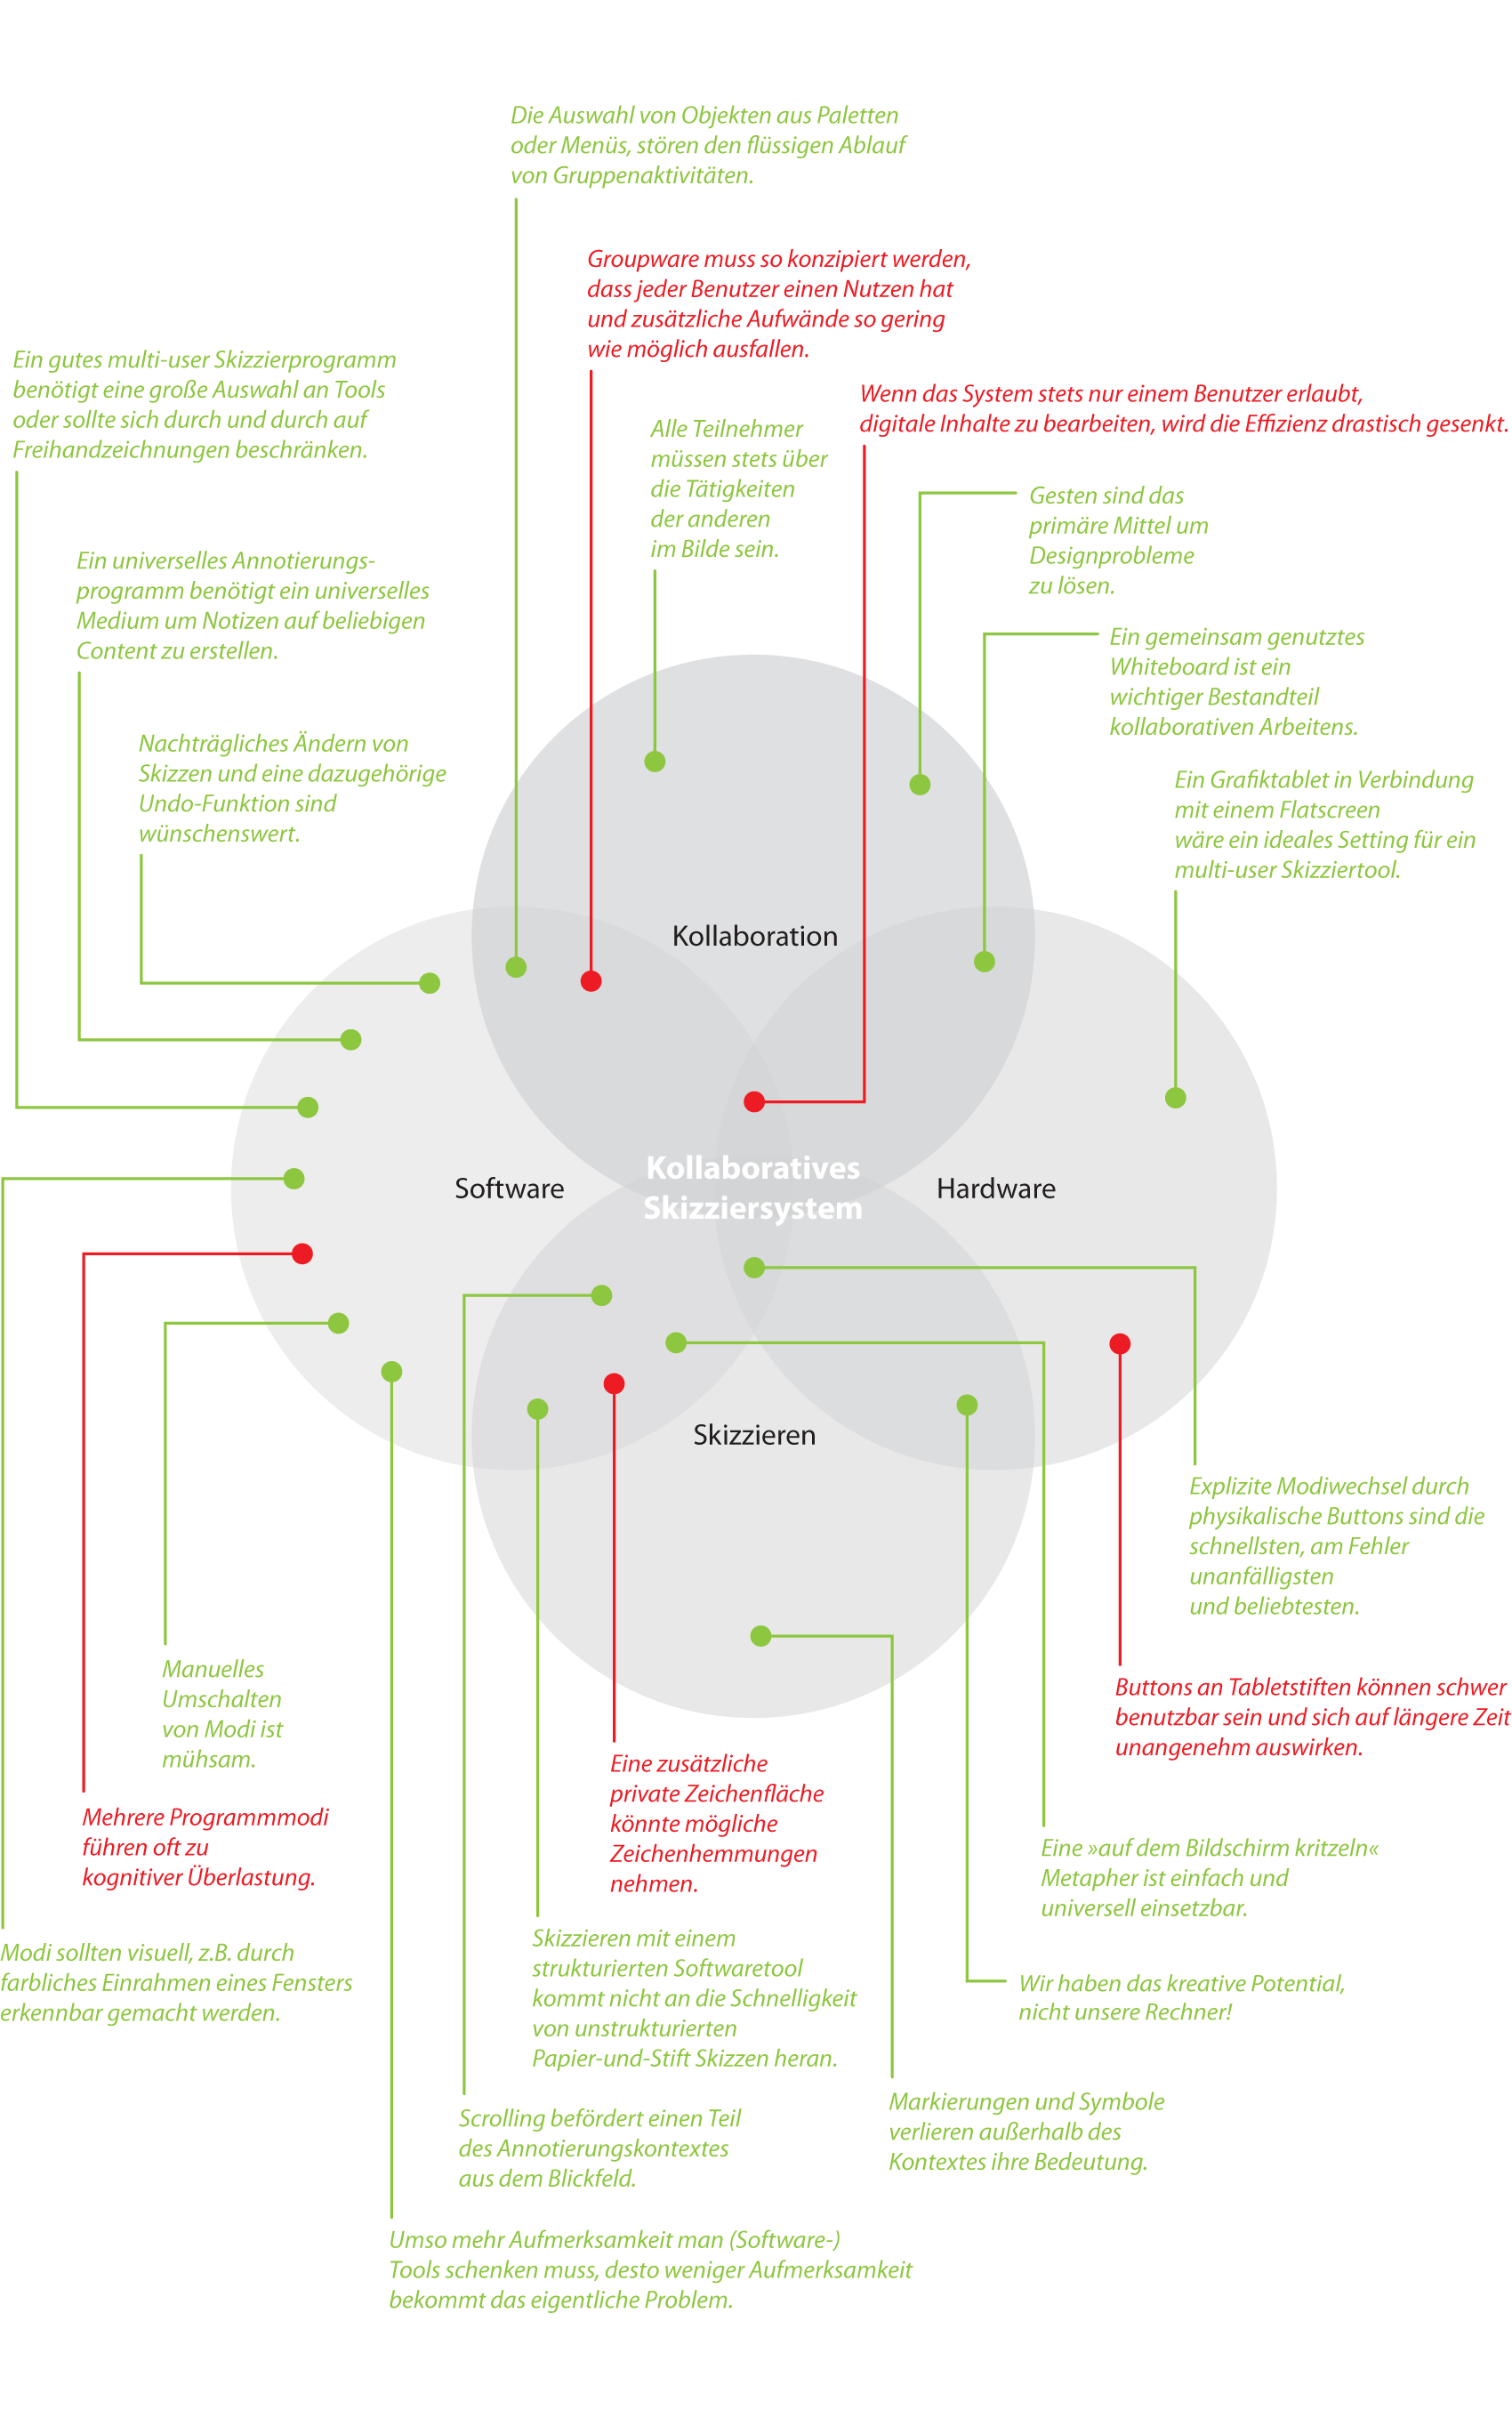
\includegraphics[bb=0cm 0cm 14.39cm 23.01cm]{gfx/scribblerAnforderungsauswertung}}
		\caption[Anforderungsauswertung für Scribbler]{Anforderungsauswertung für Scribbler. Alle umgesetzten Anforderungen sind in Grün gehalten. (Noch) nicht umgesetzte Anforderungen sind rot markiert.}\label{fig:scribblerAnforderungsauswertung}
\end{figure}

\section*{Zusammenfassung}
lorem ipsum